%%
%% This is file `sample-sigconf.tex',
%% generated with the docstrip utility.
%%
%% The original source files were:
%%
%% samples.dtx  (with options: `sigconf')
%% 
%% IMPORTANT NOTICE:
%% 
%% For the copyright see the source file.
%% 
%% Any modified versions of this file must be renamed
%% with new filenames distinct from sample-sigconf.tex.
%% 
%% For distribution of the original source see the terms
%% for copying and modification in the file samples.dtx.
%% 
%% This generated file may be distributed as long as the
%% original source files, as listed above, are part of the
%% same distribution. (The sources need not necessarily be
%% in the same archive or directory.)
%%
%% The first command in your LaTeX source must be the \documentclass command.
\documentclass[sigconf]{acmart}

%%
%% \BibTeX command to typeset BibTeX logo in the docs
\AtBeginDocument{%
  \providecommand\BibTeX{{%
    \normalfont B\kern-0.5em{\scshape i\kern-0.25em b}\kern-0.8em\TeX}}}

%% Rights management information.  This information is sent to you
%% when you complete the rights form.  These commands have SAMPLE
%% values in them; it is your responsibility as an author to replace
%% the commands and values with those provided to you when you
%% complete the rights form.
\setcopyright{acmcopyright}
\copyrightyear{2018}
\acmYear{2018}
\acmDOI{10.1145/1122445.1122456}

%% These commands are for a PROCEEDINGS abstract or paper.
\acmConference[Woodstock '18]{Woodstock '18: ACM Symposium on Neural
  Gaze Detection}{June 03--05, 2018}{Woodstock, NY}
\acmBooktitle{Woodstock '18: ACM Symposium on Neural Gaze Detection,
  June 03--05, 2018, Woodstock, NY}
\acmPrice{15.00}
\acmISBN{978-1-4503-XXXX-X/18/06}


%%
%% Submission ID.
%% Use this when submitting an article to a sponsored event. You'll
%% receive a unique submission ID from the organizers
%% of the event, and this ID should be used as the parameter to this command.
%%\acmSubmissionID{123-A56-BU3}

%%
%% The majority of ACM publications use numbered citations and
%% references.  The command \citestyle{authoryear} switches to the
%% "author year" style.
%%
%% If you are preparing content for an event
%% sponsored by ACM SIGGRAPH, you must use the "author year" style of
%% citations and references.
%% Uncommenting
%% the next command will enable that style.
%%\citestyle{acmauthoryear}


\input{libpaper/texheader}

\usepackage[normalem]{ulem}
\microtypecontext{spacing=nonfrench}

\usepackage{listings}
\usepackage{listings-rust}
\usepackage[scaled=0.85]{beramono}
\usepackage[T1]{fontenc}
\usepackage{hyperref}
\usepackage{xcolor}
\usepackage{amsthm}
\usepackage{amsmath}
\usepackage{amssymb}
\usepackage{multirow}
\usepackage{float}

\newtheoremstyle{invar}% name of the style to be used
  {0.1ex}% measure of space to leave above the theorem. E.g.: 3pt
  {0.1ex}% measure of space to leave below the theorem. E.g.: 3pt
  {\em}% name of font to use in the body of the theorem
  {0pt}% measure of space to indent
  {\bf}% name of head font
  {:}% punctuation between head and body
  { }% space after theorem head; " " = normal interword space
  {}% Manually specify head

  
\theoremstyle{invar}
%\theoremstyle{goal}
\newtheorem{invar}{Invariant}
\newtheorem{goal}{Design Goal}

\usepackage{listings-rust}

\lstset{
    language=Rust, 
    style=boxed,
    basicstyle=\ttfamily,
    columns=fullflexible,
    breaklines=true,
    escapechar=\#,
    postbreak=\mbox{\textcolor{blue}{$\hookrightarrow$}\space},
}
\lstset{language=Rust, style=colouredRust}
\lstdefinestyle{nonumbers}{numbers=none}
\newcommand{\hllr}[1]{\makebox[0pt][l]{\color{red!15}\rule[-3pt]{#1}{10pt}}}
\newcommand{\hll}[1]{\makebox[0pt][l]{\color{green!15}\rule[-3pt]{#1}{10pt}}}
\newcommand{\hlw}[1]{\makebox[0pt][l]{\color{green!35}\rule[-3pt]{#1}{10pt}}}
\newcommand{\hlc}[1]{\makebox[0pt][l]{\color{red!25}\rule[-3pt]{#1}{10pt}}}
%\remarkfalse
%\cutforspacetrue

%auto-ignore

\newcommand{\papertitle}{\This{}: Statically-Enforced Persistent Memory Safety}

\newcommand{\this}{Corundum}
\newcommand{\This}{Corundum}
\newcommand{\lst}{\mathcal{L}}


%\lstMakeShortInline!

\lstnewenvironment{rust}{}{}


\newfloat{lstfloat}{t}{lop}
\floatname{lstfloat}{Listing}

%tighten bold paragraph
\renewcommand{\boldparagraph}[1]{\vspace*{0.5ex}\noindent\textbf{#1}\hspace{1em}}


\newenvironment{goaltrue}[1]{\begin{discuss}[Design Goal~\ref{#1} (\nameref{#1}) Holds:]}{\end{discuss}}% ignore macros

\newenvironment{discuss}[1][Details:]{\boldparagraph{#1}}{\vspace{1ex}}%$\blacksquare$}

\newcommand{\rerr}{{\color{red}\textbf{{\fontencoding{U}\fontfamily{futs}\selectfont\char 66\relax}}}}

\newcommand{\refl}[1]{Line~\ref{#1}}% ignore macros ignore misc
\newcommand{\reflr}[2]{Lines~\ref{#1}--\ref{#2}}% ignore macros ignore misc


\usepackage{adjustbox}
\usepackage{array}

\newcolumntype{R}[2]{%
    >{\adjustbox{angle=#1,valign=m,height=#2,padding*=0em -1.1em 0 0.2em}\bgroup}%
    l%
    <{\egroup}%
}
\newcolumntype{K}[2]{%
    >{\adjustbox{angle=#1,valign=m,height=(#2),padding*=0em -1.1em 0 0.2em}\bgroup}%
    l%
    <{\egroup}%
}
\newcommand*\rot{\multicolumn{1}{R{40}{2em}}}% no optional argument here, please!
\newcommand*\up{\multicolumn{1}{R{90}{2em}}}% no optional argument here, please!
\newcommand*\upr{\multicolumn{1}{K{90}{2em}|}}% no optional argument here, please!


%%
%% end of the preamble, start of the body of the document source.
\begin{document}

\title{\papertitle}

\author{Morteza Hoseinzadeh}
\affiliation{%
  \institution{University of California, San Diego}
  \streetaddress{9500 Gilman Dr.}
  \city{San Diego}
  \state{California}
  \country{USA}
  \postcode{92093}
}
\email{mhoseinzadeh@cs.ucsd.edu}

\author{Steven Swanson}
\affiliation{%
  \institution{University of California, San Diego}
  \streetaddress{9500 Gilman Dr.}
  \city{San Diego}
  \state{California}
  \country{USA}
  \postcode{92093}
}
\email{swanson@cs.ucsd.edu}

%%
%% By default, the full list of authors will be used in the page
%% headers. Often, this list is too long, and will overlap
%% other information printed in the page headers. This command allows
%% the author to define a more concise list
%% of authors' names for this purpose.
\renewcommand{\shortauthors}{Trovato and Tobin, et al.}


%\title{Sustainable Persistent Programming in Rust with \This{}}


%auto-ignore
\begin{abstract}

Fast, byte-addressable, persistent main memories (PM) make it possible to
build complex data structures that can survive system failures.  Programming for PM is challenging, not least because it combines well-known programming challenges like locking, memory management, and pointer safety with novel PM-specific bug types.  It also requires logging updates to PM to facilitate recovery after a crash.  A misstep in any of these areas can corrupt data, leak resources, or prevent successful recovery after a crash.
Existing PM libraries in a variety of languages -- C, C++, Java, Go -- simplify some of these problems, but they still require the programmer to learn (and flawlessly apply) complex rules to ensure correctness.  Opportunities for data-destroying bugs abound.

This paper presents \this{}, a Rust-based library with an idiomatic PM
programming interface and leverages Rust’s type system to statically avoid most
common PM programming bugs.  \This{} lets programmers develop persistent data
structures using familiar Rust constructs and have confidence that they will be free of those bugs.
We have implemented \this{} and found its
performance to be as good or better than Intel's widely-used PMDK~\cite{pmdk} library, HP's Atlas~\cite{atlas},
Mnemosyne~\cite{mnemosyne}, and go-pmem~\cite{gopmem}.
    
\end{abstract}



%%
%% The code below is generated by the tool at http://dl.acm.org/ccs.cfm.
%% Please copy and paste the code instead of the example below.
%%
\begin{CCSXML}
  <ccs2012>
   <concept>
    <concept_id>10010520.10010553.10010562</concept_id>
    <concept_desc>Computer systems organization~Embedded systems</concept_desc>
    <concept_significance>500</concept_significance>
   </concept>
   <concept>
    <concept_id>10010520.10010575.10010755</concept_id>
    <concept_desc>Computer systems organization~Redundancy</concept_desc>
    <concept_significance>300</concept_significance>
   </concept>
   <concept>
    <concept_id>10010520.10010553.10010554</concept_id>
    <concept_desc>Computer systems organization~Robotics</concept_desc>
    <concept_significance>100</concept_significance>
   </concept>
   <concept>
    <concept_id>10003033.10003083.10003095</concept_id>
    <concept_desc>Networks~Network reliability</concept_desc>
    <concept_significance>100</concept_significance>
   </concept>
  </ccs2012>
\end{CCSXML}

\ccsdesc[500]{Computer systems organization~Embedded systems}
\ccsdesc[300]{Computer systems organization~Redundancy}
\ccsdesc{Computer systems organization~Robotics}
\ccsdesc[100]{Networks~Network reliability}

%%
%% Keywords. The author(s) should pick words that accurately describe
%% the work being presented. Separate the keywords with commas.
\keywords{datasets, neural networks, gaze detection, text tagging}

%%
%% This command processes the author and affiliation and title
%% information and builds the first part of the formatted document.
\maketitle

%auto-ignore
\section{Introduction}
\label{sec:introduction}

Persistent main memory (PM) is the first new memory technology to arrive in
the memory hierarchy since the appearance of DRAM in the early 1970's.  PM offers
numerous potential benefits including improved memory system capacity,
lower-latency and higher-bandwidth relative to disk-based storage, and a unified programming model for
persistent and volatile program state.  However, it also poses a host of novel
challenges.  For instance, it requires memory controller and ISA support, new operating
system facilities, and it places large, novel burdens on programmers.

The programming challenges it poses are daunting and stem directly from its
non-volatility, high-performance, and direct connection to the processor's
memory bus.  PM's raw performance demands the removal of system
software from the common-case access path, its non-volatility requires that (if
it is to be used as storage) updates must be robust in the face of system failures,
and its memory-like interface forces application software to deal directly with issues
like fault tolerance and error recovery rather than relying on layers of system software.

In addition, programming with PM exacerbates the impact of existing types of
bugs and introduces novel classes of programming errors.  Common
errors like memory leaks, dangling pointers, concurrency bugs, and data structure corruption have
permanent effects (rather than dissipating on restart).
New errors are also possible: A programmer might forget to log an update to a
persistent structure or create a pointer from a persistent data structure to
volatile memory.  The former error may manifest during recovery
while the latter is inherently unsafe since, after restart, the pointer to
volatile memory is meaningless and dereferencing it will result in (at best) an
exception.

The challenges of programming \emph{correctly} with PM are among the largest
potential obstacles to wide-spread adoption of PM and our ability to fully
exploit its capabilities.  If programmers cannot reliably write and modify code
that correctly and safely modifies persistent data structures, PM will be
hobbled as a storage technology.

Some of the bugs that PM programs suffer from have been the subject of
years of research and practical tool building.  The solutions and approaches to
these problems range from programming disciplines to improved library support
to debugging tools to programming language facilities.

% \remark{Some more elegant words}

Given the enhanced importance of memory and concurrency errors in PM
programming, it makes sense to adopt the most effective and reliable mechanisms
available for avoiding them.

The Rust programming language provides programming language-based mechanisms to
avoid a host of common memory and concurrency errors.  Its type system,
standard library, and ``borrow checker'' allow the Rust compiler to statically
prevent data races, synchronization errors, and memory
allocation errors.  Further, the performance of the resulting machine code is
comperable with that of compiled C or C++.  In addition to these built-in
static checks, Rust also provides facilities that make it easy (and idiomatic)
to create new types of smart pointers that integrate cleanly with the rest of
the language.  Its type systems also make data modification explicit and easy to control.

We have leveraged Rust's abilities to create \this{}, a library (or ``crate''
in Rust parlance) that lets programmers build persistent data structures.
\This{} provides basic PM programming facilities (e.g., opening and mapping
persistent memory pools) and a persistent software transactional memory
interface to provide atomic updates to persistent data.

Uniquely, \this{} uses (mostly) static checking to enforce several key PM
programming invariants:

\begin{itemize}
 
\item \This{} prevents the creation of unsafe pointers between non-volatile memory regions (or ``pools'') and pointers from those pools into volatile memory.
  
\item \This{} ensures that programs only modify persistent memory within transactions and that they log all updates to persistent state.
  
\item \This{} prevents persistent memory allocation errors (leaks, dangling pointers, and multiple frees) in the presence of multiple, independent pools of PM.
  
%\item \This{} hides low-level PM programming operations (e.g. preserving write ordering, creating logs, etc.) behind its high-level interface.

\end{itemize}

Our experience building \this{} demonstrates the benefits that a strong type
system can bring to PM programming.  We evaluate \this{} quantitatively and
qualitatively by comparing it to existing PM programming libraries.  We find
that \this{} provides stronger guarantees than other libraries and that it is
as fast or faster than those libraries.  We also highlight some changes
to Rust that would make \this{} even more powerful and efficient.

The rest of paper is organized as follows. \refsec{sec:background} gives a brief
background information on PM programming and the Rust language.
\refsec{sec:overview} describes \this{}.  In \refsec{sec:results}
we evaluate our library. \refsec{sec:related} places \this{} in context relative to related work.
 Finally, \refsec{sec:conclude} concludes.

% \remark{Mention lower level PM programming constructs}

% \remark{Mention learning curve shifting}




%auto-ignore
% -*-  eval: (display-line-numbers-mode 1)(auto-fill-mode 1); -*-
\section{Background}
\label{sec:background}

\this{} adds PM programming support to Rust by providing facilities for
accessing persistent memory, providing a transaction mechanism to ensure
consistency in the case of failure, and statically detecting common PM
programming bugs.

To accomplish this, \this{}  confronts a set of challenges that are common
among PM programming systems for languages like C, C++, and Java.
\This{} addresses these challenges using the unique features of Rust.


\subsection{Persistent Memory Programming}
\label{sec:prog}

The emergence of persistent main memory technologies (most notably Intel's
Optane DIMMs)~\cite{3DXPoint} brings byte-addressable, persistent memory to
modern processors.  The persistent memory appears in the processor's physical
address space.

The most popular operating system mechanism for exposing persistent memory to
applications is to use a PM-aware file system to manage a large region of
persistent memory.  An application can use a direct access (DAX) \mmap{} system
call to map a file in the file system into its virtual address space.  From
there, the application can access the memory directly using load and store
instructions, avoiding all operating system overheads in the common case.

\subsubsection{PM Programming Support}

While DAX \mmap{} provides access, productively and safely using PM presents
challenges that typical PM programming libraries address.  To be
successful, \this{} must address these as well.  Below, we outline the most
important of these challenges.
  

PM libraries provide access to
multiple independent \emph{pools} of persistent memory with a \emph{root} object
from which other objects are reachable.

Each pool has a private, atomic memory
allocator for allocating and reclaiming space within the pool that is robust in the face of system crashes.

Libraries usually identify which types can
exist in a pool.  For instance, the library may provide a base class or interface that
persistent object should inherit from or implement.

Finally, PM libraries provide a means to express atomic sections, usually in
the form of a persistent software transactional
memory~\cite{pmdk,nvheaps,oracle-nvm-direct} mechanism that specifies regions of code
that should be atomic both with respect to failure and to concurrent
transactions.

\subsubsection{PM Bugs}

PM programmers must reckon with a wide range of potential bugs that can cause
permanent corruption, lead to unsafe behavior, or leak resources.  These
include common memory allocation/deallocation errors and race conditions as
well as PM-specific challenges.  

The three most critical types of PM-specific bugs are logging errors, unsafe
inter-pool pointers, and pointers into closed pools.

\boldparagraph{Logging errors} An atomic section
must log all persistent updates so the transaction can roll back in
case of a system failure~\cite{nvheaps,pmfs,atlas,mnemosyne,aries,rewind}.  Failing to manually log an update (as some
systems require) can let a poorly-timed system crash compromise data integrity.

Updates can be hard to recognize in code, leading to unlogged updates.  For instance,
passing the address of a field of a persistent struct to a library function
might (to the programmer's surprise) modify the data it points to.

\boldparagraph{Inter-pool pointers} PM programs can simultaneously access
several, independent PM pools in addition to the conventional, volatile heap
and stack.  The PM pools need to be self-contained so that one pool does not
contain a pointer into another pool or into volatile memory.  Dereferencing
such a pointer is certain to be unsafe after a restart.

\boldparagraph{Pool Closure} If a pool closes, the system must unmap
the memory it contains.  This leaves any pointers from DRAM into the pool unsafe~\cite{nvheaps}.



\subsection{Rust}
\label{sec:rust}

The Rust programming language~\cite{rustbook} is intended for parallel,
low-level, systems programming and it uses a sophisticated type system to
prevent a range of common programming errors.  For instance, its type system 
makes data races impossible and it provides cheap reference counting garbage collection.
The result is a thoroughly modern language that is about as fast
as C or C++ but with vastly stronger safety guarantees.

Rust is a well-loved by the developers who use it~\cite{mostloved} despite having
a moderately steep learning curve due to it requiring
programmers to think differently about variable lifetimes, mutability, and
concurrency.

Since the memory allocation, synchronization, and safety invariants that PM
programming provides are a strict superset of those for conventional volatile
programming, we can leverage Rust's safety guarantees to improve the safety of
PM programming.

Many guarantees that Rust provides are not built in the
language itself, but are implemented in its standard library.  This means that
we can use the same language features to enforce new guarantees in an idiomatic
and familiar (to Rust programmers) way.

Below we, describe the key features of Rust that \this{} uses to provide
PM-specific safety guarantees.  For a thorough introduction, consult the Rust manual~\cite{rustbook}.

\subsubsection{Mutability, Immutabilty, and Interior Mutability}

Mutability is a central concept in Rust that governs when a value may change.
The critical property that Rust maintains is that there can be one mutable
reference to a piece of data or multiple immutable references, but not both.
We refer to this as \emph{the mutability invariant}.  In most instances, Rust
enforces this invariant statically.

\ignore{In some cases, static checks are too restrictive or the program may need to
enforce further constraints on when data can be mutable.  For
instance, Rust's \csym{Mutex} is a container that holds the data it protects.
It enforces mutual exclusion by preventing the creations of references (mutable
or immutable) to its contents if another thread holds the mutex.

\csym{Mutex} illustrates the important concept of \emph{interior mutability}.
Curiously, \csym{Mutex} objects themselves are always immutable.  However,
\csym{Mutex} exposes a mutable reference to its contents using interior
mutability: \csym{Mutex.lock()} can return a mutable guard object that is a
reference to data the mutex contains and protects.  When the guard goes out of
scope, the lock is released.}

In some cases, static checks are too restrictive or the program may need to
enforce further constraints on when data can be mutable.  Rust provides
\emph{interior mutability} for these situations, and the wrapper type
\csym{RefCell} exemplifies this concept.  Curiously, \csym{RefCell}s are always
immutable so assigning to them directly is impossible.  However, the program
can acquire mutable and immutable references by calling
\cfunc{RefCell::borrow\_mut} and\linebreak\cfunc{RefCell::borrow}, respectively.  These
functions return reference objects (similar to smart pointers) that programs
can use to access the data.  The key is that the \csym{RefCell}
dynamically enforces the mutability invariant: Calling \cfunc{borrow} when a
mutable reference object exists or \cfunc{borrow\_mut} when any reference object
exists will cause a \cfunc{panic!}.


%\This{} uses interior mutability to prevent modifications to presistent data
%outside of transactions.

\subsubsection{Smart Pointers, Wrappers, and Dynamic Memory Allocation}
\label{sec:wrapper}

Rust uses smart pointers and type wrappers to implement memory management,
garbage collection, and concurrency control.  Defining new kinds of smart
pointers, type wrappers, and guard objects that integrate cleanly into the language is easy,
since Rust makes dereferencing smart pointers fully transparent.

Rust's standard library provides a range of smart pointer types and type
wrappers (the \csym{<>} notation is Rust's syntax for generics):

\begin{enumerate}

\item \csym{Box<T>} is a pointer to an object of type \csym{T} allocated on a
  the heap.  When a \csym{Box<T>} goes out of scope, the allocated data is
  freed.
  
\item \csym{Rc<T>} is a reference-counted pointer to a heap-allocated object of type
  \csym{T}.  Multiple instances of
  \csym{Rc<T>} can point to the same data, and when the last \csym{Rc<T>} goes
  out of scope, the data is reclaimed.  Since multiple
  \csym{Rc} instances can refer to the same data, \csym{Rc<T>} does not allow
  the modification of data it holds.

\item \csym{RefCell<T>} (described above) is a wrapper type holds an object of type \csym{T} that
  is immutable except via interior mutability.

\item \csym{Mutex<T>} is a thread-safe version of \csym{RefCell}.  Its
  \cfunc{lock} method, locks the mutex and returns a reference object that is
  also a guard object for the mutex.  When the reference goes out of scope, the
  lock is released.
  
%\item \csym{Option<T>} is a value that can either hold a value of type \csym{T}
%  or no value at all (i.e, \csym{None}).

%% \item \csym{UnsafeCell<T>} is Rust's primitive to support interior mutability.
%%   All interior mutability is ultimately implemented in terms of
%%   \csym{UnsafeCell<T>}.

%% \item \csym{Cell<T>} allows by-value read/write operations using
%%   \cfunc{get}/\cfunc{set} functions with interior mutability.
  
\end{enumerate}

Each of these wrappers encapsulates a specific set of capabilities, and
programmers can compose them to build feature-rich data types.  For instance, a
common idiom -- \csym{Rc<RefCell<T>{>}} -- combines \csym{RefCell}
with \csym{Rc} to provide shared, mutable objects.
%\steve{(Arc and RefCell are not composable. The correct composition is either 
%\csym{Rc<RefCell>} or \csym{Arc<Mutex>})} 

\cutforspace{For instance,
the type \csym{Rc<RefCell<u32> >} is a modifiable, reference-counted pointer
to a heap-allocated unsigned 32-bit integer.  Note that while \csym{Arc} does
not provide mutable access to the \csym{RefCell},
the \csym{RefCell} \emph{does} allow mutable access via interior mutability.
For instance, \csym{Option<Box<u32> >} is non-reference counted pointer that
can be null.}

When the last reference to an object dies, Rust ``drops'' it.  Dropping a
struct recursively drops
any fields it contains and types can implement \cfunc{drop} to implement destructor-like
functionality.  For instance, \cfunc{drop} for \csym{Box} deallocates the
memory it holds, and \cfunc{drop} for \csym{Rc} decrements the reference
count and frees the memory if it reaches zero.

\subsubsection{Option Types}

Rust provides optional values in form of\linebreak\csym{Option<T>} that can be either \csym{Some(data)} (where \csym{data} is of type \csym{T}), or \csym{None}.  Its most common use to allow for null pointers: \csym{Box<T>} is always a valid pointer to allocated memory, but \csym{Option<Box<T{>}>} can either be \csym{None} or a \csym{Box<T>}.


\csym{Option} is one instance of Rust's \csym{enum} mechanism, and Rust provides a \csym{match} construct that is similar to \csym{switch} in C, but requires the programmer provide code for all possible values.  For \csym{Option<PBox<T{>}>}, this avoids null dereferences and forces code to account for pointers that might be null.

\cutforspace{

  \subsubsection{Ownership and Borrowing}
\label{sec:scope}

The notion of ``ownership'' is central to Rust's ability to statically avoid data races and unsafe pointer dereferences.  At any time, each value in Rust has a single variable that ``owns'' it.  When the owner goes out of scope, the value is dropped and its resources can be reclaimed.  Programs can transfer ownership through variable assignment or by passing the variable to a function.

In addition to simple variables, Rust also supports ``references'' that can refer to values without owning them.  Passing a reference to a function causes the function to ``borrow'' the value from the caller.  While the value is borrowed, the owner cannot access it.

By default, variables and references are immutable, and programmers must take explicit action to create mutable variables and references.  Further, only a single mutable reference can exist at any time.
}

\ignore{\This{} exploits these constraints to prove safety in \refsec{sec:sys}}

\ignore{To better manage the memory, languages define the scope of visibility of an object.  Rust enforces a set of rules, called ``Scoping Rules'' to manage memory and shield the program against resource leak bugs. Scopes indicate to the compiler when variables are created or destroyed, when resources can be freed, and when borrows (we will discuss borrowing later in this section) are valid. These rules consider variables owning resources. Using RAII, Rust compiler instruments destruction code whenever the object goes out of its scope, frees resources belonging to it, and invalidates borrows.}

\ignore{\subparagraph{Ownership.} To prevent data races and provide memory safety, Rust variables are considered as the owners of resources. Enforced by RAII, they are in charge of freeing their own resources when they are not in use. To prevent multiple deallocation, resources can only have one owner. Therefore in Rust's design, the ownership of data is transferred to the new variable instead of simply copying data in a data assignment operation (e.g. \csym{let x = y}). This is also happening when we pass an argument to a function. In that case, the scope of the data also changes to the internal scope of the function, because the original variable is no longer owning the resource. Changing the ownership of data also determines its mutability state. When a resource is owned by an immutable variable, its content cannot be changed. }

\ignore{\subparagraph{Borrowing.} Taking the ownership of data is not always useful, especially when we would like to access data temporarily in another function. To realize this, Rust comes with a borrowing mechanism that allows passing resources by reference (\csym{\&T}). The compiler uses a borrow checker to statically guarantee the validity of referents. Just like moving the ownership, values also can be borrowed with different mutability options. If a value is moved immutably, there is no way to modify it. Rust also prevents mutable referencing an immutable variable to prevent data race. There can be one or more immutable references to a resource (\csym{\&T}), or exactly one mutable one (\csym{\&mut T}), but it is not possible to have both types at the same time. Data can be borrowed again when the mutable reference no longer exists. When a mutable data is immutably borrowed, it cannot be modified via the original owner until all references go out of scope.}

\ignore{\subparagraph{Lifetime.} To prevent access violation while lending out a reference to a resource in another scope, Rust defines lifetime for every reference. Lifetime (or \textit{borrow checker}) determines when a borrow is available, and when a resource can be borrowed. A good example of that is when we attempt to return a reference to a local variable in a function. Rust compiler prevents this case because the lifetime of the local variable is the internal scope of the function which is smaller than the lifetime of its borrow that is being sent out from the function scope.}

\ignore{
and traits (similar
to Java interfaces).  It does not support inheritance.


}

\subsubsection{Traits and Type Bounds}
\label{sec:gen}

Rust provides \emph{traits} that are similar to Java or C\# interfaces.
Structures can implement traits.  A ubiquitous Rust idiom is to ``bound'' or
restrict the types that can be used in a particular context based on the traits
they implement. 

Of particular importance are ``auto traits'' that all types (even primitive types)
implement by default but can opt out of.  For instance, all types
implement the \csym{Send} trait so they can be sent to another thread.
Rust allows negative implementation (using \csym{!} symbol) of auto traits for
opting out of it. For instance, \csym{Rc<T>} is labeled as 
\csym{!Send} because it uses non-atomic counters and is, therefore, not safe to share among threads.

\ignore{\subsubsection{Concurrency}

Rust's provide built-in support for threads and its type system eliminates
data races.  Two traits -- \csym{Sync} and
mark types that be shared between threads and allow Rust to enforce the mutability
invariant across threads.}

\subsubsection{Panic}

In response to serious errors, programs can call\linebreak\cfunc{panic!} to end the
program.  Rust provides an exception-like mechanism to catch panics and attempt
to recover from them.

\subsubsection{Unsafe Rust}

Rust provides \csym{unsafe} code blocks which give the programmer access to a
superset of normal, safe Rust.  Unsafe Rust
allows C-like direct manipulation of memory, unsafe casts, etc.  The Rust
standard library uses unsafe Rust to implement interior mutability and many
other critical features (e.g., system calls and low-level memory management).

Libraries like \this{} can declare types or functions to be unsafe, preventing
their invocation or use in safe code.

If programmers decide to use \csym{unsafe} constructs, they
assume responsibility for enforcing the guarantees that Rust (or the library)
relies upon.  Typical Rust programmers do not use
\csym{unsafe} constructs.

\cutforspace{\subsubsection{Standard Library}

The Rust standard library provide efficient implementations of vectors, hash
maps, and strings.  These implementation make use of unsafe code to improve
performance.
}

\ignore{\subsubsection{Copy and Clone Traits}

For safety reasons, Rust does not copy smart pointers upon assignment operations to avoid multiple untraceable references to a memory location. To provide referencing to an owned memory locations, pointer types implement the \csym{Clone} trait. The programmer can copy the memory location (for \csym{Box<T>}), or instantiate a new reference (for \csym{Rc<T>} and \csym{Arc<T>}) by explicitly invoking the \csym{clone} function. \this{} provides \csym{PClone} as an alternative for \csym{Clone} trait in PM.
}

\ignore{\subsubsection{Option Type}

Rust provides optional values in form of \csym{Option<T>} that can be either \csym{Some(data)}, or \csym{None}. It has several uses in Rust including, but not limited to, nullable pointers. Since the smart pointer types cannot be assigned to null values, wrapping them in an \csym{Option} is a solution to represent a nullable smart pointer. Similarly, \this{} provides \csym{MaybeNull} (either \csym{Valid(data)} or \csym{Null}) which implements \csym{PClone} as opposed with \csym{Clone} in \csym{Option}.}

% \morteza{If you are going to use \csym{None} and \csym{Some} you need to describe what they are.} \steve{I didnt get it. Isnt it clearto show enough?}

\ignore{\subsubsection{Interior Mutability}

To strongly reason about pointer aliasing, Rust disallows multiple mutable references to a shared object. However, this limits the flexibility of having pointers to a shared data. To allow mutation, Rust provides \csym{Cell} and \csym{RefCell} types which allow mutable access to the interior data even though the they are not mutably referenced. \csym{Cell} allows updating data through the \cfunc{set} function without borrowing it mutably, and \csym{RefCell} allows mutable borrowing by enforcing Rust's ownership rules at runtime. Neither of these violates Rust's safety rules.}

\ignore{\subsubsection{Chain Drop}
\label{sec:chain}

Rust enforces RAII (Resource Acquisition Is Initialization) that invokes the destructor of data when its owner goes out of scope before freeing the resources. Rust makes sure that all dependent objects are dropped prior to the object itself. This creates a finite chain of calls to the destructors and properly reclaiming the allocated memory. However, data is not really a dependent in pointer objects. Therefore, Rust provides \csym{Drop} trait that allows types performing more operations while being dropped. Using which, the pointer types can branch the dropping chain to include their referents too. More specifically, \csym{Box} always extends dropping to its pointee, while \csym{Rc} and \csym{Arc} do this only when they find no strong reference to the data. 
}


%% Important points

%% \begin{enumerate}
%% \item Pointer safety and Pool Containment
%%   \begin{enumerate}
%%   \item No null pointer dereference (Rust)
%%   \item No inter-pool pointers \nameref{inv:no-interpool-ptrs}
%%   \item No NV-to-V pointers \nameref{inv:no-v-pointers}
%%   \end{enumerate}
%% \item Transactions
%%   \begin{enumerate}
%%   \item Atomicity \nameref{inv:tx-atomic}
%%   \item Consistency \nameref{inv:inevitable-logging}
%%   \item Isolation (Rust)
%%   \item Durability ***
%%   \item all of the above for volatile data too.
%%     \begin{enumerate}
%%     \item Atomicity \nameref{inv:tx-no-volatile-mutability}
%%     \item Consistency \nameref{inv:inevitable-logging}
%%     \item Isolation (Rust)
%%     \end{enumerate}
%%   \end{enumerate}
%% \item Memory safety
%%   \begin{enumerate}
%%   \item No memory leaks. \nameref{inv:no-orphans}
%%   \item No multiple frees. \nameref{inv:correct-gc}
%%   \end{enumerate}
%% \item Concurrency
%%   \begin{enumerate}
%%   \item No data races. (Rust)
%%   \item No unsynchronized access. (Rust)
%%   \end{enumerate}
%% \end{enumerate}

%auto-ignore
\lstMakeShortInline^

\section{\This}
\label{sec:overview}

\This{} is a Rust library (or ``crate'') that uses static and dynamic checking to avoid common PM programming errors.
Aside from providing these strong safety guarantees, \this{} 
is similar to other PM programming libraries like
PMDK~\cite{pmdk}, NV Heaps~\cite{nvheaps}, and Mnemosyne~\cite{mnemosyne}.
\This{} provides four abstractions -- typed persistent memory pools,
transactions, persistent smart pointers, and atomic memory allocation -- that
address the challenges and common bugs described in \refsec{sec:prog}.

\This{} strives to provide strong safety guarantees for persistent memory programming.
It achieves the following design goals:


%% \begin{itemize}

%%   \myitem{Transactions and Atomic Memory Management} All modification to
%%   persistent data (including memory allocation) occur within transactions.
%%   \This{} enforces this constraint statically making a pool's journal object
%%   available inside transactions and no where else.

%%   \ignore{\This{} enforces this constraint by requiring all mutating,
%%     allocating, and deallocating operations to take a journal object (of type
%%     \csym{Journal<P>}) as a parameter.  Journal objects are only available
%%     inside transactions and cannot escape.}

%%   \myitem{Leak-Free Memory Allocation} To prevent persistent memory leaks,
%%   \this{} statically ensures that, by the end of the enclosing transaction, any
%%   allocated memory has either been reclaimed or been made reachable from the
%%   root of the memory pool.

%%   \myitem{Logging errors} Journal objects record mutating operations made during a
%%   transaction, so they can roll back in case of a system failure or
%%   transactions abort.  Since all mutating operations require a journal object,
%%   it is not possible to accidently omit an update from the journal.

%%   \myitem{Inter-pool pointers} Since the type of each persistent pointer and
%%   object includes a pool type, \this{} can prevent inter-pool pointers by
%%   disallowing assignments between different pool types.
  
%% \end{itemize}


%% \begin{enumerate}
%% \item Pointer safety and Pool Containment
%%   \begin{enumerate}
%%   \item No null pointer dereference (Rust)
%%   \end{enumerate}
%% \item Transactions
%%   \begin{enumerate}
%%   \item Atomicity \nameref{inv:tx-atomic}
%%   \item Consistency \nameref{inv:inevitable-logging}
%%   \item Isolation (Rust)
%%   \item Durability ***
%%   \item all of the above for volatile data too.
%%     \begin{enumerate}
%%     \item Atomicity \nameref{inv:tx-no-volatile-mutability}
%%     \item Consistency \nameref{inv:inevitable-logging}
%%     \item Isolation (Rust)
%%     \end{enumerate}
%%   \end{enumerate}
%% \item Memory safety
%%   \begin{enumerate}
%%   \item No memory leaks. \nameref{inv:no-orphans}
%%   \item No multiple frees. \nameref{inv:correct-gc}
%%   \end{enumerate}
%% \item Concurrency
%%   \begin{enumerate}
%%   \item No data races. (Rust)
%%   \item No unsynchronized access. (Rust)
%%   \end{enumerate}
%% \end{enumerate}


\begin{goal}[Only-Persistent-Objects]
  Pools only contain data that can be safely persistent.\label{goal:only-persistent-objects}
\end{goal}
\begin{goal}[Ptrs-Are-Safe]
  Pointers within a pool are always valid.  Pointers between pools or from
  persistent memory to volatile memory are not possible.  Pointers from
  volatile memory into a pool are safe.  Closing a pool does not result in
  unsafe pointers.\label{goal:ptrs-are-safe}
\end{goal}
\begin{goal}[Tx-Are-Atomic]
  Transactions are atomic with respect to both persistent and volatile data.
  It is not possible to modify persistent data without logging
  it.\label{goal:atomic-is-atomic}
\end{goal}
\begin{goal}[No-Races]
  There are no data races or unsynchronized access to shared persistent data. \label{goal:no-races}
\end{goal}
\begin{goal}[Tx-Are-Isolated]
  Transactions provide isolation so that updates are not visible until the transaction commits. \label{goal:atomic-is-isolated}
\end{goal}
\begin{goal}[No-Acyclic-Leaks]
  Memory leaks in acyclic data structures are not possible. \label{goal:no-memory-leaks}
\end{goal}
%\begin{goal}[No-NV-to-V-Ptr]
%  \This{} pools do not contain pointers to volaitle memory.  \label{goal:no-pool-to-dram-ptr}
%\end{goal}
%\begin{goal}[V-to-P-Ptrs-Are-Safe]
%  \This{} pools do not contain pointers to volaitle memory.  \label{goal:no-pool-to-dram-ptr}
%\end{goal}
%\begin{goal}[Inevitable-Logging]
%  Modifying data without logging the change is not possible. \label{goal:inevitable-logging}
%\end{goal}
%\begin{goal}[No-Null-Deference]
%  Null pointer derefence is not possible. \label{goal:no-null-dereference}
%\end{goal}

\This{} achieves these goals through a combination of several core techniques
that are embodied by \this{}'s abstractions.  \This{} borrows and relies
upon existing features of Rust to prevent data races and avoid unsafe pointer
manipulation.  These properties are a foundation that \this{} builds upon.

\this{} breaks a program's execution into transactions and non-transactional
code, and a thread's execution alternates between the two.  Transactions are atomic,
isolated, and can modify persistent state but cannot modify pre-existing
volatile state.  The remaining, non-transactional code
can modify volatile state but cannot modify persistent state.

Critically, \this{} limits the kinds of variables that can cross transaction
boundaries, and this allows for careful reasoning about the invariants that
hold at the boundaries.  For instance, \this{} guarantees that leaks are not
possible by showing that they do not exist at transaction boundaries.

\subsection{Assumptions}

\ignore{The correctness of \this{} builds on many features of Rust and its safety
properties.  In particular we rely directly on Rust to satisfy two of our
design goals: \nameref{goal:no-memory-leaks} and \nameref{goal:no-races}.  The
Rust documentation~\cite{rustbook} details of how Rust provides these
guarantees.}

The correctness of \this{} rests on several assumptions.
We assume that the program does not use \csym{unsafe} constructs, since
unsafe Rust can bypass almost all of the guarantees that Rust makes and relies
upon.  \ignore{\This{} also prohibits spawning threads inside a transaction, for reasons discussed in \refsec{sec:discuss}.}

We also assume that our implementation of the \this{} memory allocator,
logging and recovery code, and reference counting system are correct.  We have
tested them thoroughly and techniques for building correct versions of these
components are well-known~\cite{nvheaps,mnemosyne,atlas,pmdk,oracle-nvm-direct}.

Finally, students of Rust will notice that we do not discuss some common types
(e.g., \csym{Cell} or \csym{Weak}) or their persistent analogs.
\This{}'s treatment of these types is analogous to the types we discuss and \this{}
provides persistent counterparts.  We have omitted the details for brevity.

\subsection{\This{} Pools and Objects}

\This{} provides self-contained pools of persistent memory and constrains the
data types that they can hold.

\boldparagraph{Pools} \This{} pools reside in a
PM-backed file.  The pool contains some metadata, a root pointer, persistent
memory allocation data structures, and a region of persistent memory.

\This{} identifies each memory pool with a \emph{pool type}, and all persistent
types take a pool type as a parameter.  This statically binds each persistent
object to its pool.  Likewise, transactions are bound to a particular pool via
the pool type.  In our discussion, we use \csym{P} as a representative pool
type.

Programs open a pool by calling \csym{P}'s \cfunc{open} function:\linebreak\csym{P::open<T>("foo")}.  This binds \csym{P} to the pool in file
\csym{foo}.  \This{} ensures that only one open pool is bound to \csym{P} at
any time.  The type parameter, \csym{T}, determines the type of the root
pointer.  \cfunc{P::open<T>} returns an immutable reference to the root pointer.  Pools remain
open until reference to the root object drops.

Programmers can statically declare multiple pool types using the
\cfunc{pool!} macro, but the number of pool types available (and,
therefore, the number of simultaneously open pools) is fixed at compile time.

\boldparagraph{Persistent Objects} Objects in a pool must implement the
\csym{PSafe} auto trait.  \This{} declares all primitive arithmetic types to be
\csym{PSafe}, so these types and structs composed of them are \csym{PSafe}.

\csym{PSafe} (like all of \this{}'s auto traits) is declared
\csym{unsafe}, so programmers should not explicitly label types as \csym{PSafe}.

Reference and raw pointers, and types that refer to state external to the program (e.g., file handles) are \csym{!PSafe}. Having a \csym{!PSafe} field (as in \csym{Box}, \csym{Rc}, \csym{Arc},
\csym{Mutex}, etc.), also, makes a type \csym{!PSafe}.

\begin{lstfloat}
  \begin{lstlisting}[escapechar=\@]
#[derive(Root)]
struct Node {
  val: i32,
  next: PRefCell<Option<Pbox<Node,P>@@>,P>
}
fn append(n: &Node, v:i32, j: &Journal<P>) {
  let mut t = n.next.borrow_mut(j);@\label{ln:borrow}@
  match &*t {@\label{ln:match}@
    Some(succ) => append(succ, v, j);
    None => *t = Some(Pbox::new(@\label{ln:new}@
        Node {
          val: v,
          next: PRefCell::new(None, j)
        }, j));
  }
}
fn go(v: i32) {
  let head = P::open::<Node>("list.pool",0);
  P::transaction(|j| {@\label{ln:tx}@
    append(&head, v, j);@\label{ln:call}@
  });@\label{ln:txend}@
}
\end{lstlisting}
\caption{A \this{} implementation of linked list append.  Some error management code has been elided for clarity.}
\label{lst:example}
\end{lstfloat}

% \begin{table*}%[!ht]
%   \center
%   \small
%   \begin{tabular}{p{3.4in}p{3.4in}}
%     \begin{lstlisting}[escapechar=\#,caption=Insert method of a sorted linked-list in Rust]
% struct Node {val:i32, nxt:Rc<RefCell<Option<Node>>>}
% impl Node {
%   fn append(&self, val: i32) {
% #\hllr{\linewidth}#
%     let mut nxt = self.nxt.borrow_mut();
%     if let Some(n) = &*nxt {
%       if n.val > val {
%         *nxt = Some(Node { val,
%           nxt: self.nxt.clone()
%         })
%       } else { n.insert(val); }
%     } else {
%         *nxt = Some(Node { val,
%           nxt: Rc::new(RefCell::new(None))})
%     }
% #\hllr{\linewidth}#
%   }
% }
% fn main() {
% #\hllr{\linewidth}#  let head = #\hlc{77pt}#Default::default();
%   head.insert(10);
% }\end{lstlisting}
%     &
%       \begin{lstlisting}[escapechar=\#,caption=Insert method of a sorted linked-list in \This,label=lst:examples]
% #\hll{\linewidth}# struct Node {val:i32, nxt:#\hlw{12pt}#Prc<#\hlw{32pt}#PRefCell<Option<Node>>>}
% impl Node {
%   fn append(&self, val: i32) {#\label{ln:tx2}#
% #\hll{\linewidth}#    #\hlw{72pt}#transaction(|j| {
% #\hll{\linewidth}#      let mut nxt = self.nxt.borrow_mut(#\hlw{5pt}#j);#\label{ln:borrow}#
%       if let Some(n) = &*nxt {#\label{ln:if}#
%         if n.val > val {#\label{ln:if2}#
%           *nxt = Some(Node { val,
% #\hll{\linewidth}#            nxt: self.nxt.#\hlw{38pt}#pclone(j)
%           })
%         } else { n.insert(val); }
%       } else {
%         *nxt = Some(Node { val,
% #\hll{\linewidth}#          nxt: #\hlw{12pt}#Prc::new(#\hlw{32pt}#PRefCell::new(None,#\hlw{5pt}#j),#\hlw{5pt}#j)})#\label{ln:new}#
%       }
% #\hll{\linewidth}#    #\hlw{47pt}#}).unwrap()#\label{ln:txend2}#
%   }
% }
% fn main() {
% #\hll{\linewidth}#  let head = #\hlw{127pt}#P::open::<Node>("list.pool",0);
%   head.insert(10);
% }\end{lstlisting}
% \end{tabular}
% \vspace*{-\baselineskip}\vspace*{-\baselineskip}
% \end{table*}


\subsection{Transactions: The Basics}

All modifications to a \this{} pool occur within a transaction, including
memory allocations and modifications of the root pointer.

Programs create transactions by passing an anonymous function (i.e., a lambda) to \cfunc{P::transaction} (\reflr{ln:tx}{ln:txend} of \reflst{lst:example}).
The lambda takes a single
argument, \csym{j}, which will be reference to a \emph{journal object} that holds information about the current transaction.  Variable
\csym{j} is of type \csym{Journal<P>}, so it is bound to pool \csym{P}.  

The lambda can capture values from the transaction's lexical scope (e.g., \csym{head} in \reflst{lst:example}), allowing
transactions to integrate smoothly into the surrounding code.
\cfunc{P::transaction} returns the return value of the transaction body.

\This{} flattens nested transactions: Modifications to a
pool commit when outermost transaction for that pool commits.  \cutforspace{This rule
holds for nested transactions on different pools, so an inner transaction on
\csym{P} will commit before an enclosing transaction on \csym{Q} finishes.   We discuss
the possibilities for multi-pool transactions in \refsec{sec:discuss}.}

The programmer is responsible for acquiring locks in the correct order to avoid deadlock.

Rust's type system allows \this{} to restrict the inputs and output of the
transaction.  The \csym{TxInSafe} auto trait bounds the types a transaction
can capture.  \This{} marks all volatile mutable references, smart pointers, wrappers,
and interior mutability types as \csym{!TxInSafe}.

This provides our first invariant:

\begin{invar}[TX-No-Volatile-Mutability]
  \label{inv:tx-no-volatile-mut}
  Transactions cannot modify existing volatile state.
\end{invar}

\begin{discuss}
  Since all the types that provide mutable access to volatile data are
  \csym{!TxInSafe}, pre-existing instances of these variables are not available
  inside the transaction (\refl{ln:txinsafe} of \reflst{lst:lifetime}).  However, 
  %moved objects (using keyword `\csym{move}') and new instances of these
  variables can be created and modified within the transaction.  Preexisting
  volatile data can be read.
  
\cutforspace{The code below illustrates the restrictions. The transaction can declare
volatile variables on the stack or heap inside the transaction (\reflr{l:createvstart}{l:createvend}),
modify them, and read captured values (\reflr{l:modifyvstart}{l:modifyvend}).
But, it cannot modify captured values (\reflr{l:unsaferef}{l:unsafebox}).  Nor
can it create a mutable reference to a captured value (\refl{l:unsafemake}).

\begin{lstfloat}
  \begin{lstlisting}
    let mut a = 42;
    let b = &mut a;
    let mut c = Box::new(42); 
    let r = P::transaction(|j| {
	let mut d = 0;             #\label{l:createvstart}#
	let mut e = Box::new(42);  #\label{l:createvend}#
	d = a;  #\label{l:modifyvstart}#
	*e = a; #\label{l:modifyvend}#
        // #\rerr{}#@*b = 0;@  #\label{l:unsaferef}#
        // #\rerr{}#*c = 0;  #\label{l:unsafebox}#
        // #\rerr{}#let g = &mut a; #\label{l:unsafemake}#
	// #\rerr{}#return e #\label{l:noreturnbox}#
	return d #\label{l:yesreturnvalue}#
    }).unwrap();
\end{lstlisting}
\end{lstfloat}

The example shows that the transaction can return newly-created volatile data
by value (\refl{l:yesreturnvalue}) but not by reference/pointer (\refl{l:noreturnbox}).}

%% \subsubsection{Durability.} Another aspect of pointer safety is that the objects they refer live longer than the static lifetime of the program, and they should be reachable when the program restarts to avoid memory leaks. Therefore, \this{} prevents moving out a pointer wrapper from the transaction that it is born in, unless there is a link from the root object to it. To implement that, we consider a special auto trait `\csym{TransactionOutSafe}' that is not implemented by the pointer wrappers. Then we bound the output types of the transaction to be marked as \csym{TransactionOutSafe}.

\begin{lstfloat}
\begin{lstlisting}
let mut done = false;
let p1 = P::transaction(|j|{
    let p1 = Pbox::new(1, j);
    let p2 = Pbox::new(2, j);
    root.set(p2);
    done = true;#\label{ln:txinsafe}#
    --^^^^ the trait `TxInSafe` is not
    --     implemented for `&mut bool`
    p1#\label{ln:p1}#
    --^^ the trait bound `Pbox<i32,P>:TxOutSafe`
    --   is not satisfied
}).unwrap();
++^ `p1` is dropped here.
++^ `p2` is alive and durable here because it
++  is reachable from the root object.
\end{lstlisting}
\caption{Reachability though lifetime and type bounding}
\label{lst:lifetime}
\end{lstfloat}
% }

%Since newly-allocated volatile memory cannot escape, it will be reclaimed when
%the transaction ends.  As a result,

\end{discuss}

\csym{TxOutSafe} bounds the values a transaction can return.  All references
and pointers are \csym{!TxOutSafe}, so transactions can return data only by
value. \refl{ln:p1} of \reflst{lst:lifetime} shows how the compiler
complains when a user attempts to send out a persistent object.

\This{} also uses the concept of a \emph{stranded type}: If a type is
\csym{!TxOutSafe}, \csym{!Send}, and \csym{!PSafe}, then instances of that type
cannot escape a transaction.  This is because 1) Since a stranded type is
\csym{!TxOutSafe}, the transaction cannot return it, 2) since it is
\csym{!PSafe}, it cannot be stored in a pool for later retrieval, 3) since it is
\csym{!Send}, it cannot be passed to another thread, and 4) it cannot be assigned 
to a volatile variable (\nameref{inv:tx-no-volatile-mut}).

%\This{} uses is this capability to enforce several invariants:

\begin{goaltrue}{goal:only-persistent-objects}
  The declaration of \cfunc{P::open} includes a bound to ensure that the root is
  \csym{PSafe}.  If it contains references or pointers they must be one of
  the persistent reference/pointer types (see below), since volatile pointers
  and references are \csym{!PSafe} (e.g. \reflst{lst:psafe}).
  
  \csym{PSafe} is a type bound on all of the persistent smart pointer and wrapper
  types, so those types can only point to, refer to, or wrap \csym{PSafe}
  objects.

\begin{lstfloat}
\begin{lstlisting}
P1::transaction(|j1| {
    let v = Box::new(10);
    let p1 =
      Pbox::new(v, j1);
                --^ Box<i32>:PSafe is not satisfied
}).unwrap();
\end{lstlisting}
\caption{Only persistent-safe objects are acceptable.}
\label{lst:psafe}
\end{lstfloat}
\end{goaltrue}

\This{} also carefully constrains the availability of journal objects:

\ignore{\begin{invar}[TX-No-PMEM-Return]
  \label{inv:tx-no-pmem-return}
  Transactions cannot return pointers or references to persistent data.
\end{invar}

\begin{discuss}
  \This{} marks all persistent pointer, reference, and wrapper types as \csym{!TxOutSafe}.
\end{discuss}
}

\begin{invar}[TX-Journal-Only]
  \label{inv:tx-journal-only} 
  Journal objects are only available inside transactions.  \cutforspace{For nested
  transactions, only the journal object for the innermost transaction is
  available.}
\end{invar}

\begin{discuss}
  The constructor for the \csym{Journal<P>} is unsafe, so the program cannot
  safely create one.  Therefore, the only journal objects that might be
  available are the ones passed to a transaction as an argument.
  \csym{Journal<P>} is declared to be stranded, so it cannot escape the transaction.
  
  \cutforspace{Finally, a nested transaction cannot capture the journal object from the outer
    transaction, because \csym{Journal<P>} is \csym{!TxInSafe}.  }
\end{discuss}

\ignore{\begin{invar}[TX-atomic]
  \label{inv:tx-atomic}
  A \this{} transaction only modifies persistent state if it commits.
\end{invar}
\begin{discuss}
  We have designed and tested our transaction implementation carefully to
  ensure that this invariant is met.
\end{discuss}
}

\subsection{Pointers to Persistent Data}

\This{}'s smart pointer, smart reference, and wrapper types play a crucial role
in avoiding persistent programming errors, since they mediate access to
persistent state.  Their design prevents pointers from one persistent pool to
another, prevents the modification of persistent state outside of transactions,
and plays a role in avoiding memory leaks.

\begin{table*}
{ \centering
  \footnotesize
  \begin{tabular}{|l|l|p{4in}|}\hline
    \this{} type              &API                                              &Description \\\hline\hline
\multicolumn{3}{|c|}{\textbf{PMEM Smart Pointers for Dynamic Allocation}}\\\hline\hline
\csym{Pbox<T,P>}         &                                                 &Statically scoped, unshared pointer to PMEM.  Deallocates when it goes out of scope.\\
                          &\csym{new(value: T, j: \&Journal<P>)}                             &Allocate PMEM in \csym{P} and initialize it.\\\hline
\csym{Prc<T,P>}           &&Dynamic PMEM allocation with thread-unsafe reference counting.\\
\csym{Parc<T,P>}         &                                                &Dynamic PMEM with thread-safe reference counting.\\
&\csym{new(value: T, j: \&Journal<P>)}                             &Allocate PMEM in \csym{P} and initialize it.\\
&\csym{pclone(j: \&Journal<P>)}&Create a new reference to the data.\\
&\csym{downgrade()->PWeak}&Return a persistent weak (\csym{PWeak<T,P>}).\\
&\csym{demote()->VWeak}&Return a volatile weak pointer (\csym{VWeak<T,P>}).\\\hline
\csym{PWeak<T,P>}&\csym{upgrade(j: \&Journal<P>)->Prc/Parc}&Convert to a \csym{Option<Prc/Parc<T,P>{>}} if it is available\\\hline
\csym{VWeak<T,P>}&\csym{promote(j: \&Journal<P>)->Prc/Parc}&Convert to a \csym{Option<Prc/Parc<T,P>{>}} if it is available\\\hline\hline
\multicolumn{3}{|c|}{\textbf{PMEM Wrappers for Interior Mutability}}\\\hline\hline
\csym{PCell<T,P>}        &                                                &Interior mutability via copying data to and from PMEM using \cfunc{get} and \cfunc{set} functions.\\
%&\csym{new(value: T, j: \&Journal<P>)}                             &Create new instance on the stack and initialize it.\\
%&\csym{get()}&Return the contents of the cell by value.\\
%&\csym{set(value: T, j: \&Journal<P>)}&Set the contents of the cell by value.\\\hline
\csym{PRefCell<T,P>}     &                                                &Interior mutability via references with dynamic borrow checking.\\
&\csym{new(value: T, j: \&Journal<P>)}                             &Create new instance on the stack and initialize it.\\
&\csym{borrow()}&Return an immutable reference to value it contains.\\
&\csym{burrow\_mut(j: \&Journal<P>)}&Return a mutable reference object (\csym{RefMut}) for the value inside.\\\hline
\csym{PMutex<T,P>}        &                                                &Thread-safe interior mutability via references.\\
&\csym{new(value: T, j: \&Journal<P>)}                             &Create new instance on the stack and initialize it.\\
&\csym{lock(j: \&Journal<P>)}&Lock and return a mutable reference (\csym{PMutexGuard}).\\\hline%\hline
%\multicolumn{3}{|c|}{\textbf{Mutable Reference Types}}\\\hline\hline
%\csym{PMutexGuard<'a, T: 'a, P>}&&Smart reference that provides interior mutability for \csym{PMutex}.\\\hline
%\csym{RefMut<'a, T: 'a, P>}&&Smart reference that provides interior mutability for \csym{PRefCell}.\\\hline

  \end{tabular}}
  \caption{\This{}'s smart pointers and type wrappers for persistent data
    corresponding closely Rust's pointers and wrappers for volatile data.  The
    key differences are that the \this{} types takes pool type as a type
    parameter, binding them to a particular pool.}
  \label{tab:types}
\end{table*}

\ignore{
  \begin{table*}
    \center
    \small
    \begin{tabular}{|l|l|p{1in}|p{1in}|}
      \hline
      &Description&\multicolumn{2}{|c|}{Key types that are...}\\
&&\csym{x}&\csym{!x}\\\hline
\csym{TxInSafe}&Types that can be captured transactions.&\csym{Pbox<T,P>}, \csym{Parc<T,P>}, \csym{Prc<T,P>}, \csym{PRefCell<T,P>}, \csym{PCell<T,P>}, \csym{Pmutex<T,P>}, \csym{RootCell<T,P>}, \csym{\&T}, primitive arithmetic types, &\csym{\&mut T}, \csym{RefCell<T>}, \csym{Cell<T>}, other mutable or interior mutable volatile types, \csym{Journal<P>}\\\hline
\csym{TxOutSafe}&Types that can be returned by transactions.&primitive arithmetic types.&\csym{Journal<T>}, \csym{Pbox<T,P>}, \csym{Parc<T,P>}, \csym{Prc<T,P>}, \csym{PRefCell<T,P>}, \csym{PCell<T,P>}, \csym{Pmutex<T,P>}, \csym{RootCell<T,P>}, \csym{\&T},\\\hline
\csym{PSafe}&Types that are allowed in persistent pools.&\csym{Pbox<T,P>}, \csym{Parc<T,P>}, \csym{Prc<T,P>}, \csym{PRefCell<T,P>}, \csym{PCell<T,P>}, \csym{Pmutex<T,P>}, \csym{RootCell<T,P>}, primitive arithmetic types.&\csym{\&T}, \csym{\&mut T}, \csym{RefCell<T>}, \csym{Cell<T>}, other references to volatile data, IO-related types (e.g., file handles), \csym{Journal<P>}\\\hline\hline
\csym{Send}&Rust type trait for values that can be transferred between threads.&Everything else&\csym{Prc<T,P>}, \csym{Journal<P>}, \csym{PRef<T, P>}, \csym{PMutRef<T, P>}, \csym{PMutexGuard}\\\hline
\csym{Sync}&Rust type trait for values that can be shared between threads.&&\\\hline

    \end{tabular}
    \caption{}
    \label{tab:traits}
  \end{table*}
}

\reftab{tab:types} summarizes \this{}'s persistent smart pointer types.  With
the exception of \csym{VWeak}, they mirror Rust's volatile smart pointers (See
\refsec{sec:background}).  The interface differs in two ways: First, each type
takes a pool type as a type parameter, so pointers that reside in different
pools have different types.  Second, their constructors and mutating accessors
take a journal object as an argument.

Three of the methods listed --
\cfunc{PRefCell::borrow},\linebreak\cfunc{PRefCell::borrow\_mut}, and
\cfunc{PMutex::lock} -- return objects that behave like references.  These
objects are all stranded. %subject to same constraints as the smart pointers (e.g., they
%are \csym{!TxOutSafe}).

\csym{VWeak} is a pointer from volatile memory into a pool.  It is ``weak'' in
the sense that it does not affect reference counts.  The \cfunc{promote} method
grants access to the data a \csym{VWeak} refers to by providing a \csym{Parc}
that refers to the same data.  Promoting is only possible within a transaction.
\cfunc{Parc::demote} creates \csym{VWeak} pointers.

\begin{goaltrue}{goal:ptrs-are-safe}
The presence of multiple pools of PM alongside the volatile heap and stack
means the potential for several different kinds of pointers, complicating 
pointer safety.

\boldparagraph{Pointers within a pool} These pointers are allowed and \this{}
relies on Rust's safety properties and mechanisms to ensure their safety.

\boldparagraph{Pointers between pools} Inter-pool pointers are inherently
unsafe.  They are not possible in \this{}, because pointers to different
pools have different types, and assignment between types is not allowed in Rust.

\cutforspace{Statically checking types in assignment is almost sufficient to prevent
  inter-pool pointers, but there is one caveat: If the programmer explicitly
 declares that a pool contains a pointer to another pool, the Rust type system
 cannot detect the error statically.
 
 For instance, consider this code:
 
 \begin{lstlisting}
   P::open::<PBox<u32, Q>, P>(...);
 \end{lstlisting}

 It declares that the root of \csym{P} is a \csym{PBox} that points to pool
 \csym{Q}.  We conisder this an error, and a simple dynamic check flags it and
 calls \csym{panic()}.

 \fixme{Is there some cool type system feature we could say would fix this problem?}
}

\boldparagraph{Pointers from a pool to volatile memory} These pointers are
also inherently unsafe.  They are also disallowed: Pools only contain
\csym{PSafe} objects (\nameref{goal:only-persistent-objects}) and pointers to
volatile memory are \csym{!PSafe}. 

\boldparagraph{Pointers from volatile memory into a pool} The object a
\csym{VWeak} refers to can disappear if the last \csym{Parc} refering to the
object goes out of scope, deallocating the memory. In this case,
\cfunc{promote} will return \csym{None}, which is safe in Rust.

\boldparagraph{Pointers into closed heaps} If a heap closes, dereferencing any
pointers into the heap becomes unsafe.  \This{} combines three approaches to
prevent this.

First, accessing a pointer to a closed pool from within a transaction is not
possible, since \cfunc{P::transaction} will \cfunc{panic!} if \csym{P} is
closed.

Second, consider a reference (other than \csym{VMWeak}, \csym{A}, that exists
outside a transaction.  Rust's borrow checker requires that chain of in-scope
references exists from the root to \csym{A}.  This includes the root pointer,
whose liveness prevents \csym{P} from closing.

Finally, \csym{VWeak} pointers from volatile memory into the pool can exist
after the pool closes.  However, \cfunc{VWeak::promote} requires a journal
object to retrieve a usable reference, so it can only be called from inside a
transaction, which is only possible if \csym{P} is open (see above).

% \subsubsection{Strong static type system.} In order to prevent cross pool referencing, we consider pools as data types, and generate new persistent pointer type for each pool. Although this constrains the pool types to be known in compile time, it provides strong safety guarantees. For example, \reflst{lst:cross} shows a code snippet in which the programmer attempts to assign an integer data allocated in \csym{P2} to a pointer existing in \csym{P1} which is prevented by the compiler. The objection is that \csym{p1} is a \csym{LogCell} that contains a pointer of type \csym{Pbox<i32,P1>} while \csym{p2} is a pointer of type \csym{Pbox<i32,P2>}.

\begin{lstfloat}
\begin{lstlisting}
P1::transaction(|j1| {
    let p1 = LogCell::new(
        Pbox::new(1, j1), j1);
    P2::transaction(|j2| {
        --^^^^^^^^^^^ `j1` is not `TxInSafe`
        let p2 = Pbox::new(1, j2);
        p1.set(p2, j1);
               --^^ expected P1, found P2
    }).unwrap();
}).unwrap();
\end{lstlisting}
\caption{Cross-Pool referencing prevention via type system}
\label{lst:cross}
\end{lstfloat}
\end{goaltrue}
  
\subsection{Transactions: Mutability and Isolation}

\This{} allows modification of persistent data only via interior mutability
and only inside a transaction.
Two wrapper types in \reftab{tab:types} provide interior mutability for persistent data:
\csym{PMutex} and \csym{PRefCell}.%, and \csym{LogCell}.

\cfunc{PMutex::lock} returns a mutable reference to the data while
acquiring a lock.  The lock is automatically release at the end of the
transaction.

\csym{PRefCell} returns mutable and immutable references via\linebreak
\texttt{PRefCell::borrow\_mut} and \cfunc{PRefCell:borrow},
respectively.  It dynamically enforces Rust's mutability
invariants for these references.

\ignore{\cfunc{PMutex::lock} and \cfunc{PRefCell::borrow\_mut} \ignore{,
  and \cfunc{LogCell::set} all} take a journal object an argument, so they
cannot be called outside a transaction (\nameref{tx-journal-only}).}

\begin{invar}[Mutable-In-Tx-Only]
  \label{inv:mutable-in-tx-only}
  Mutable references to persistent data in \csym{P} can only exist inside transactions on \csym{P}.
\end{invar}

\begin{discuss}
  The program can create a mutable reference to persistent data by calling
  \cfunc{borrow\_mut} or \cfunc{lock} on a smart pointer.  Since both of
  these functions require a journal object as a parameter, they can only be called inside a
  transaction (\nameref{inv:tx-journal-only}).

  The resulting mutable reference object (either a \csym{PRefMut} or a
  \csym{PMutexGuard}) is stranded, so it will be destroyed when it goes out of
  scope at the end of the transaction.
  
  The reference that \cfunc{open} returns to the root object is immutable, so
  initially, there are no mutable references to pool data available outside a
  transaction.

  Since new mutable references that a transaction creates are stranded, the
  number of such references outside a transaction cannot increase, so there
  will never be such a reference.
\end{discuss}

\begin{goaltrue}{goal:atomic-is-atomic}
  For persistent data, \This{}'s atomicity guarantee relies on the atomicity of
  the memory allocator and on all modifications to persistent data being
  logged.

  The allocator and journal object ensure that allocations do not become
  persistent until the transaction commits.  Therefore, on a system failure or
  \cfunc{panic!}, the allocations roll back to reclaim the allocated memory.  \ignore{We
  discuss the allocator implementation in \refsec{sec:impl}.}
  
  \This{} enforces logging by requiring a journal object to make changes to
  data.  To modify persistent data, the program needs a mutable reference
  object from \csym{PRefCell::borrow\_mut()} or \cfunc{PMutex::lock}.  The
  reference object performs undo logging the first time it is dereferenced.

  %We discuss the implementation of the
  %logging and recovery mechanism in \refsec{sec:impl}.  We have tested it
  %thoroughly to ensure its correctness.

  Atomicity should include updates to volatile state as well, since
  a transaction can abort if it calls \cfunc{panic!}.  \This{} transactions are
  trivially atomic for volatile state because they cannot modify volatile state
  (\nameref{inv:tx-no-volatile-mut}).

%  \This{} does not make provisions for rolling back (or preventing) IO operations inside transactions.
\end{goaltrue}

\begin{goaltrue}{goal:no-races}
  Rust prevents data races and unsynchronized access using the mutability
  invariant, the \csym{Mutex} type, marker types to restrict data movement between threads.
  \This{} takes the same approach by providing \csym{PMutex}, and achieves the
  same safety guarantees.
  
\ignore{  Rust provides the \csym{Sync} traits to limit which types can be shared
  between threads.  If a type is \csym{!Sync}, only one thread may hold a
  reference to it any time.

  \csym{PMutex} is the only \csym{Sync} type that \this{} provides.  Therefore,
  any shared persistent data must be sent between threads wrapped in a
  \csym{PMutex} and the threads must take the mutex to gain read or write access.}
\end{goaltrue}

\begin{goaltrue}{goal:atomic-is-isolated}
  Isolation requires that changes in an uncommitted transaction are not visible
  to concurrently executing code.

  Since transactions cannot modify shared volatile data
  (\nameref{inv:tx-no-volatile-mut}), we only need to consider changes to
  persistent objects.

  A thread must hold a lock before reading or writing shared persistent state
  and this can only occur inside a transaction
  (\nameref{inv:tx-journal-only}).  Once a thread holds the mutex, no other
  thread can read the data it protects until the transaction commits and the lock is released, so other threads are isolated from
  those changes.
\end{goaltrue}

\subsection{Memory Management}

\This{} constrains where programs can allocate and deallocate persistent memory
and provides an allocator that can atomically commit or roll back all the
allocations and deallocation that occur in a transaction.

\This{} adopts Rust's reference counting garbage collection mechanism.
\csym{Parc} and \csym{Prc} smart pointers provide
 persistent reference counting.  \This{} (and Rust)
also support weak references to allow for cyclic data structures.

Like Rust's \csym{Rc} and \csym{Arc},  \csym{Prc} and \csym{Parc} provide
a cloning method, \cfunc{pclone}, to create a new strong reference to the shared
data and increment the reference count.  The reference counts are persistent, so
modifying them requires \cfunc{pclone} to take a journal object.

\boldparagraph{Allocation} The only way to allocate persistent memory is by
creating \csym{Pbox}, \csym{Prc}, or \csym{Parc} instances.  Since the
constructors for these types require a journal object, allocation cannot
occur outside a transaction.

\ignore{\begin{invar}[Alloc-Is-Atomic]
  \label{inv:alloc-is-atomic}
  If a transaction does not commit, any allocations or deallocations it performed are rolled back.
\end{invar}

\begin{discuss}
  The allocator and journal object ensure that allocations do not become
  persistent until the transaction commits.  Therefore, on a system failure or \cfunc{panic},
  the allocations roll back to reclaim the allocated memory.  We discuss the
  allocator implementation in \refsec{sec:impl}.
\end{discuss}}

\boldparagraph{Deallocation} When a reference count goes to zero (for
\csym{Prc} or \csym{Parc}) or a \csym{Pbox} goes out of scope, the variable is
``dropped'' signifying that the allocator can reclaim the memory.  However,
instead of releasing it immediately, \this{} logs the release and performs it
during transaction commit.

Logging occurs in \cfunc{drop} (i.e., the destructor) for \csym{Prc},
 \csym{Parc} and \csym{Pbox}.  \This{} must ensure that
deallocation only occurs within a transaction.

This guarantee holds since the destruction of an object only occurs in response to a change in another
persistent object (e.g., the destruction of the last reference to that
object).  Since \this{} only allows changes to persistent memory inside
transactions (\nameref{inv:mutable-in-tx-only}), the resulting object
destruction will occur in the same transaction.

\cutforspace{
\fixme{i do not know what this invariant is for, but i find it comforting.  i think it eliminates a bunch crazy things you could do in \csym{drop}}

\begin{invar}
  The \cfunc{drop} method for persistent objects cannot modify any persistent
  data other than the object being dropped.
\end{invar}

\begin{discuss} 
The \cfunc{drop} method takes a mutable reference to \csym{self} as its only
argument, and the method can use the reference to modify the fields of
\csym{self}.

However, it cannot gain mutable access to anything else.  This is because
\csym{self} is the only persistent object or reference available.  While
\csym{self} may contain smart pointers to persistent state, gaining mutable
access to those objects requires a journal object.  No journal object is
initially available inside \cfunc{drop}.

Starting a transaction inside \cfunc{drop} will provide access to a journal object,
but the mutable reference to \csym{self} is \csym{!TxInSafe}, so it is
unavailable inside the transaction.
\end{discuss}
}

\subsection{Memory Allocation}
\label{sec:rev:alloc}

\This{} extends Rust's reference-counting memory management system to prevent persistent memory
leaks (in the absence of cycles) and multiple-frees.
\This{} provides an additional guarantee that is necessary for persistent memory: It ensures that, by the end of the allocating transaction, the newly allocated persistent memory is reachable from some previously allocated persistent memory.  This ensures that crashes (which
invalidate all volatile pointers) do not leak volatile memory.

\begin{goaltrue}{goal:no-memory-leaks}

\This{} adds three mechanisms extending Rust's reference counting mechanism to prevent memory leaks in acyclic persistent data structures.
First, the atomicity of memory allocations within a transaction prevents the
creation of orphaned data if a transaction does not commit.  Second, the
transaction cannot assign a newly-allocated PMEM region to a captured volatile
variable (\nameref{inv:tx-no-volatile-mut}).  This prevents persistent data
from being kept alive solely by a volatile reference.  Third, since the
persistent pointers types are \csym{!TxOutSafe}, PMEM data cannot escape the
transaction via the transaction's return value.

As a result, the only way a new PMEM allocation can outlive the transaction is
to become reachable from a region of persistent memory that was allocated
in an earlier transaction. 

\cutforspace{\begin{invar}[Ref-Count-Works]
  \label{inv:refcount}
  \This{}'s reference counting garbage collector works correctly.
\end{invar}

\begin{discuss}
  For this discussion below, we assume that \this{}'s reference counting system and memory allocator are implemented correctly.  For the reference counter, this means that it only reclaims a block when the reference count goes to zero.  For the allocator, correct operation requires that it can perform multiple allocations and deallocations atomically as part of a transaction.  For both, we assume that they recover correctly after a crash occurs during a transaction, so that the reference counting and memory allocation state after recovery is logically equivalent to what it had been before the failed transaction began.
\end{discuss}
}


  
\ignore{We begin by dividing \csym{P}'s allocatable space (i.e., excluding per-pool
metadata) into \emph{blocks}.  Every block is in one of two states:
\emph{allocated} or \emph{free}.

A block, \emph{B} is \emph{reachable} from another block \emph{A}, if \emph{A}
contains a \csym{Pbox}, \csym{Prc}, or \csym{Parc} that points to \emph{B} or
another block, \emph{C} such that \emph{B} is reachable from \emph{C}.  Further
assume there are no cycles among the pointer in \csym{P}.

%\csym{P} is \emph{flawless} if the following condition holds for every block in \csym{P}:  The block is either 1) allocated and reachable from the the root of \csym{P} \emph{or} 2) free and not reachable from the root.  If a block violates this condition, then we say it is a \emph{flaw} or is \emph{flawed}.

We proceed by induction on the number of transactions executed for \csym{P}
over its entire lifetime, including system failures, recoveries, and
restarts.  Initially, all of \csym{P}'s blocks are free and there are no orphans.

Since transactions roll back on failure, failed transactions cannot create
orphans.

To show that a \this{} transaction that commits does not create an orphan, consider a newly
created \csym{Pbox}, \csym{B}, in an orphan-free pool, \csym{P}.

We need to show that either \csym{B} becomes reachable
in \csym{P} \emph{or} that all references to \csym{B} go out of scope
at the end of transaction, so the memory that \csym{B} references will be
reclaimed.  That is, we must show that if \csym{B} is
not dead at the end of the transaction, it is reachable from the root
of \csym{P}.

We can assume \csym{B} is live throughout the transaction, otherwise it will be
dropped and its memory reclaimed.  Consider two possibilities: First, \csym{B} could be \emph{non-locally
live} so that it is reachable via a variable that the transaction captured.
Alternately, \csym{B} could be \emph{locally live} and be reachable \emph{only}
via variables that are local to the transaction (i.e., not reachable via any
non-local reference).

At the end of the transaction, if \csym{B} is \emph{locally live}, then all the
references to it will go out of scope when the transaction ends, and \this{}
will reclaim \csym{B}'s memory.  The only potential escape would be for the
transaction to return \csym{B} or a locally live reference to \csym{B} but \csym{B} is \csym{!TxOutSafe}, so that is impossible.

If \csym{B} is non-locally live, the transactions must have made it so by
assigning it to a variable, \csym{A}, that is reachable from a captured
variable.  Only persistent captured variables can be modified in a transaction
(\nameref{inv:tx-no-volatile-mut}), so \csym{A} must be persistent.

\csym{A} cannot be an orphan since we assumed (inductively) that there were no
orphans before the transaction started.  Therefore \csym{A} is reachable from
the root and now so is \csym{B}.
}

\ignore{
  \textbf{Limitation:} \This{} inherences the memory leak problem of reference counting from Rust. A cyclic reference (in \csym{Prc} and \csym{Parc}) leads to memory leak as the number of references never reaches zero. Therefore, the Rust programmer should be more precautious to prevent reference cycles since the are permanent.
}

The argument above hinges on the invariant that a reference to orphaned memory
cannot exist outside a transaction.  However, Rust's mechanism for spawning a
new thread provides a potential escape.  Consider this example:

\begin{lstlisting}
  P::transaction(|j| {
    let a = Parc::new(j, 42);
    thread::spawn(move |k| {
      let b = a;
    });
  });
\end{lstlisting}

Rust's \cfunc{thread::spawn} function executes its argument\linebreak
(a lambda) in a new thread.
In the code, \csym{a} is an orphan but it moves to the thread's scope.
The thread's body is outside the transaction, so our invariant does not hold.
To restore the invariant, additional to \csym{Prc}, \this{} makes \csym{Pbox}
and \csym{Parc} \csym{!Send}, too.  This prevents their capture by a thread body
or moving to the thread's scope.

\ignore{\nameref{goal:no-memory-leaks} only holds for acyclic data structures,
since \csym{Parc} and \csym{Prc} use simple reference counts and cannot detect
cycles.  If cycles exist, \this{} can leak memory although no more so than Rust
itself can.}

\ignore{Unfortunately, this prevents a thread from ever passing one of these types to
another thread.  To rectify, this \csym{Parc} provides \cfunc{pack} method
which safely encapsulates the \csym{Parc} for transport to another thread.  The
other thread can \cfunc{unpack} the encapsulated \csym{Parc}, but it must done
inside a transaction and \cfunc{unpack} does not return until the origin
transaction either commits or aborts.  If the transaction commits,
\cfunc{unpack} returns a \csym{Parc}.  If it aborts, \cfunc{unpack} returns
\csym{None}.

Using this mechanism, the above code becomes:}

\ignore{ \begin{lstlisting}
   P::transaction(|j| {
     let a = Parc::new(j, 42).pack(j);
     spawn(|| {
       P::transaction(|k| {
         let b = a.unpack(k);
       });
     });
   }) 
 \end{lstlisting}
}
\end{goaltrue}



\cutforspace{
\subsection{Cross-Pool Atomicity}

Atomically updating data in multiple pools is tricky as both pools should commit the changes at the same time. A crash may happen anytime between opening a transaction in the first pool and committing the last one. To make that possible, \this{} provides \textit{chaperoned session}s in which a third independent persistent object monitors all transactions in the session. This object is called \csym{Chaperon} and resides in a separate file. 

It contains a checklist that indicates which one of the participating transactions is committed.
When a pool initiates a transaction, it first checks whether it is called from a chaperoned session. If so, it passes its finalization functions to the chaperon instead of invoking them at the end of transaction, and notifies the chaperon when finishes. At the end of the session, the chaperon object executes the finalization functions. After executing the last one, the chaperon call it a completed session and deletes the associate file. % \reffig{fig:cross} shows the process of atomically moving an integer from one pool to another pool, leaving the first pool with value zero. When a crash happens in the gray area, both transactions roll back even when the crash is after the atomic section of \csym{P2}. If the crash happens after the gray area, it means that both of them are completed and it is safe to discard associated journals.
}

\subsection{Example}

\reflst{lst:example} implements \cfunc{append} for a persistent linked list in \this{}.  A \csym{Node} contains an integer and a link to the next \csym{Node}.  The link is of type \csym{PRefCell<Option<Pbox<Node,P>{>,P>}}, which might seem daunting, but this is typical for a Rust pointer declaration.  To break it down: \csym{PBox<Node, P>} is pointer to a \csym{Node} in pool \csym{P}.  \csym{Option<>} allows the pointer to be \csym{None}.  Wrapping the \csym{Option} in \csym{PRefCell} allows for modification via interior mutability.

The function \cfunc{append} recursively finds the end of the list \csym{n}, and adds a \csym{Node}.  \refl{ln:borrow} uses \cfunc{PRefCell::borrow\_mut} to get a mutable reference, \csym{t}, to the \csym{Option} object the \csym{PRefCell} contains. \refl{ln:match} uses Rust's \csym{match} construct to safely handle all possible values of \csym{t}: \csym{None} or \csym{Some}.  In the \csym{Some} (i.e., non-null) case, it binds the content of the \csym{Option} (which has type \csym{Node}) to \csym{succ}, and recursively calls \cfunc{append}.

If the \csym{Option} is \csym{None}, the code has reached the end of the list.  Line~\ref{ln:new} creates a \csym{PBox} to allocate a new \csym{Node} with value \csym{v} and a \csym{next} pointer equal to \csym{None}.  It wraps the \csym{PBox} in a non-null value of type \csym{Option}, and assigns it to the mutable reference.


Function \cfunc{go} opens ``list.pool'' and binds it to pool type \csym{P}.  The root pointer will hold a \csym{Node} struct.  \refl{ln:tx} starts a transaction, which provides a journal object, which \refl{ln:call} passes to \cfunc{append}.

Several aspects of the code are notable.  First, \csym{head} and \csym{n} are both immutable, so changes are not possible until \cfunc{borrow\_mut} uses interior mutability to return a mutable reference object.  Second, we must pass \csym{j} into \cfunc{append} to ensure it executes in a transaction thereby allowing the call to \cfunc{borrow\_mut}  and the memory allocation (\refl{ln:new}).  Third, although we create call \cfunc{borrow\_mut} for every link in the list, \this{} only logs the last one, since logging only happens when \csym{*t} dereferences the reference object (\refl{ln:new}).  Forth, as written, \csym{Node} and \csym{append} only work on pool type \csym{P}.  A more complete implementation would make \csym{P} a generic type parameter, so they could work on any pool type.

\newcommand{\Dynamic}{D}
\newcommand{\Static}{S}
\newcommand{\Manual}{M}

\begin{table*}
  \center
  \footnotesize
  \begin{tabular}{|l|c|c|c|c|c|c|c|c|}\hline
    %&How does it ensure that only persistent data types reside in persistent memory?&How does it prevent (or ensure the validity of) pointers from one NV region/pool to another region/pool?&How does it prevent pointers from an NV region into DRAM?&How does it ensure the safety of pointers from DRAM to NV?  For example, if an NV object's reference count goes to zero and it is deallocated or the persistent region is unmapped, how do you prevent dereferences to the resulting invalid pointers in volatile memory?&How does it prevent unsynchronized access to shared persistent data?&How does it prevent unlogged writes to persistent data?&How does it prevent modifications to persistent data outside of transactions?&How does it prevent persistent memory leaks?
System&\rot{\hyperref[goal:only-persistent-objects]{Only-P-Object}}&\multicolumn{2}{c}{\nameref{goal:ptrs-are-safe}}&&\up{\nameref{goal:no-races}}&\multicolumn{2}{c}{\nameref{goal:atomic-is-atomic}}&\rotr{\hyperref[goal:no-memory-leaks]{No-Leaks}}\\
&&Interpool&NV-to-V&V-to-NV&&Atomicity&Isolation&\\\hline\hline
NV-Heaps~\cite{nvheaps}&\Manual{}&\Dynamic{}&\Static{}&\Manual{}&\Static{}&\Static{}&\Manual{}&RC\\\hline
Mnemosyne~\cite{mnemosyne}&\Manual{}&\Dynamic{}&\Static{}&\Manual{}&\Static{}&\Static{}&\Manual{}&\Manual{}\\\hline
PMDK (libpmemobj)~\cite{pmdk}&\Manual{}&\Dynamic{}&\Manual{}&\Manual{}&\Manual{}&\Manual{}&\Manual{}&\Manual{}\\\hline
PMDK (libpmemobj++)~\cite{pmdk}&\Manual{}&\Dynamic{}&\Manual{}&\Manual{}&\Manual{}&\Static{}&\Manual{}&\Manual{}\\\hline
NVM Direct~\cite{oracle-nvm-direct}&\Dynamic{}&\Dynamic{}&\Static{}&\Dynamic{}&\Manual{}&\Static{}/\Manual{}&\Static{}/\Manual{}&\Manual{}\\\hline
Atlas~\cite{atlas}&\Manual{}&\Manual{}&\Manual{}&\Manual{}&\Manual{}&\Static{}&\Manual{}&GC\\\hline
go-pmem~\cite{atlas}&\Manual{}&\Manual{}&\Manual{}&\Manual{}&\Manual{}&\Static{}&\Manual{}&GC\\\hline\hline
Corundum&\Static{}&\Static{}/\Dynamic{}&\Static{}&\Dynamic{}&\Static{}&\Static{}&\Static{}&RC\\\hline

  \end{tabular}
  \caption{\This{} more static checks than other PMEM libraries, using them to meet most of its design goals. ('S'=Static, 'D'=Dynamic, 'M'=Manual, 'GC'=Garbage Collection, 'RC'=Reference Counting)}
  \label{tab:libs}
  \vspace{-0.5cm}
\end{table*}

\subsection{Limitations and Potential Improvements to Rust}
\label{sec:discuss}

\This{}'s design statically prevents many but not all bugs that might occur in
persistent programs.  The design decisions of Rust also impact \this{}'s design
and place some limits on what it can achieve.

\boldparagraph{Uncaught Bugs} \This{} aims to protect the programmer from
errors that violate the basic rules of persistent memory programming as
enshrined in its design goals.  However, \this{} does not attempt to protect
against higher level errors (e.g., whether a persistent hash map will function
correctly).

\boldparagraph{Dynamic Checks} In some cases, \this{} provides dynamic, rather than static, checks.
In these cases we could not find a way to enforce them with Rust's
type system.

\This{} performs dynamic checks to protect
against unsafe dereferencing of \csym{VWeak} pointers from DRAM into PM that can arise when a pool
closes.  Dereferencing these pointers is common -- imagine a volatile index
that stores pointers to persistent objects -- so static checks would be
preferable.  An enhanced version Rust's lifetime mechanism might be of use in
this case, since it might be able to keep the pool open until all pointers into
it went out of scope.

\ignore {
  \This{} also cannot prevent the declaration of a pointer from one pool to another (e.g.,
  \csym{PBox<PBox<T,Q>,P>}).  The resulting pointer is unsafe, and preventing
  such an assignment requires a dynamic check.  One solution would be to allow
  auto traits to take parameters, so a trait
  \csym{PSafe<P>} could indicate persistent safety only in pool \csym{P}.

  \steve{It might not prevent the declaration, but by making the journal object to pass the transaction boundaries, it statically prevents initialization of such type.}
}

\boldparagraph{Threads in Transaction}
\This{} goes through some contortions to make it safe to spawn a thread inside a
transaction, since there is no way to restrict where thread spawning is
possible.  The challenge is that \cfunc{thread::spawn} may leak an unreachable \csym{Parc} when called in a transaction.  To prevent this, \csym{Parc} is \csym{!Send}, which requires using \csym{Parc::VWeak} to pass persistent pointers to child threads, which is cumbersome.

A solution would be to generalize Rust's ability to bound the variables that a
transaction can capture to include functions.  We could then
make \cfunc{thread::spawn} \csym{!TxInSafe} to prevent the transaction from
calling it.

\boldparagraph{Deadlock} \This{} does not prevent deadlock despite several
demonstrations that this is possible in a TM
system~\cite{convoider,grace,tm2c,stmlock}.  We did omitted deadlock detection and
recovery for simplicity and to align \csym{PMutex}'s behavior with \csym{Mutex}'s.
  
\boldparagraph{Log-Free Programming} \This{} is more restrictive than most
existing PM libraries.  For instance, many high-performance PM data structures
are log-free and use carefully-ordered updates to ensure crash consistency.
More permissive libraries allow this, but such code would not compile under
safe \this{}.  Ideally, \this{} could grow to include
\csym{unsafe} facilities that allow for log-free programming without completely
sacrificing its safety properties.

\boldparagraph{Cyclic References} Like all reference-counting memory management systems, Rust (and \this{}) can leak memory in cyclic data structures.  The consequences are more severe for \this{}, since the memory is persistent.  Several solutions are possible (e.g., a more general garbage collection mechanism), but they would increase complexity, reduce performance, and create a mismatch between \this{}'s behavior and Rust's.

\boldparagraph{Other Languages} We chose Rust as the basis for \this{} after
considering several alternatives.  C is notoriously unsafe.  Well-behaved C++
code is an improvement and NV-Heaps and the \csym{libpmemobj}'s C++ bindings
demonstrate that C++ smart pointers and lambdas can provide some of \this{}'s
checks, but there are several significant gaps.  For instance, there is no way
to limit the types a lambda can capture.

Go~\cite{golang} emphasizes simplicity and go-pmem~\cite{gopmem} provides basic
PMEM programming facilities.  However, Go does not allow smart pointers or
provide a sufficiently expressive type system to statically enforce the
invariants that \this{} provides.

Pony~\cite{pony} is a new language with similar design goals to Rust.  For
instance, it has a sophisticated notion of mutability and statically prevents
data races, just as Rust does.  However, Pony is less mature and more complex
than Rust.

\subsection{What is Essential and What Is Rust?}

The biggest open question for \this{} is what aspects of its design (and our
correctness argument) are byproducts of choosing Rust and which represent
something more fundamental about persistent memory safety.

For instance, \this{} is unique among PMEM libraries in separating code that
modifies persistent state from code that modifies volatile state.  Our
correctness argument relies on this property in several places, but it is not
clear whether this is a fundamentally good idea for PMEM programming or simply
something that was helpful in ensuring safety and implementable in Rust.

It would be instructive to try to replicate \this{}'s functionality in another
language.  C++ seems like the most likely mainstream candidate, since it has a flexible
type system.  Simplying recreating \this{}'s approach in C++ would require
first recreating the Rust memory safety guarantees that \this{} relies on.
This seems challenging.  More illuminating would be to try to achieve the same
goals using a more idiomatic C++ approach.  A comparison between the resulting
system and \this{} would be revealing.

\ignore{


The requirements for persistent programming can be categorized into functionality and safety. The functionality requirements are the basic features that a programming language provides to enable using the persistent memory, such as allowing system calls to file operations and \mmap{} functions, and low-level implementation of cache flushing. Alternately, a PL can hide the functionalities using a persistent type abstraction.

The safety features, on the other hand requires additional layers of evaluating the program and enforcing some safety rules either statically or dynamically. Code transformation is one of the common practices to enforce safety dynamically using transactional memory and undo logging~\cite{gopmem,atlas}. However, static checking for PM safety using transactional memory and undo logging requires some linguistic support for persistent data.

Some PM programming tools add some compiler passes to instrument the code in order to add this support to the language~\cite{gopmem,atlas,autopersist,mnemosyne,oracle-nvm-direct}. Doing so requires maintaining the tool forever as the standard version of the compiler evolves. Other tools prefer using the available programming features of a language and human efforts to provide safety~\cite{pmdk}. We found the best practice to be using available PL with the following minimal features to provide PM safety statically:

\begin{itemize}
  \item \textbf{Type bounding}: Some data types, such as raw pointers, are unsafe to reside in the PM unless it is guaranteed that they point to the same memory region as they reside. Type bounding can filter out unsafe types in generics.
  \item \textbf{Explicit dereferencing}: The PL should provide a feature to distinguish between reading and writing accesses. Only when an object is accessed mutably, it can be written onto. This is useful in taking an undo log before mutation.
  \item \textbf{Type bounded $\lambda$-function}: Transactions should be able to accept closures as the failure-atomic operation, and capture only PM-safe types. Capturing variable unsafe variables may lead the program to an inconsistent state.
  \item \textbf{Garbage collection}: Objects should either have a precise lifetime or be accurately garbage collected to avoid manual deallocation.
\end{itemize}
}

%  \begin{enumerate}
%\item Rust vs. Pony vs. Go vs. c++ vs. C -- other languages for systems programming
%\item Core mechanisms in \this{}:  Restricting persistent mutability.  Controlling what pointers can point to persistent state.  Restricting how data can escape a transaction.


  
%\item Spawning thread in transactions can allow volatile data to escape.
%\item Multi pool transactions
%\item Have to open transaction to read data (i.e., to unlock a mutex)
%\item \csym{VCell<T>}
%\item thread spawning and multi-threaded transactions.
%\item We could probably build safe inter-pool pointer types.
%\item How do we prevent IO?
%\item No volatile pointers to persistent state.  No volatile index to persistent data.  Could be fixed with a better reference counting implementation.
%\item deadlock is still possible.
%\end{enumerate}

%%%%%%%%%%%%%%%%%%%%%%%%%%%%%%%%%%%%%%%%%%%%%%%%%%%%%%%%%%%%%%%%%%%%%%%%%%%%%%%%%%%%%%%%%%%%%%%%%%%%%%%%%%%%
%%%%%%%%%%%%%%%%%%%%%%%%%%%%%%%%%%%%%%%%%%%%%%%%%%%%%%%%%%%%%%%%%%%%%%%%%%%%%%%%%%%%%%%%%%%%%%%%%%%%%%%%%%%%
%%%%%%%%%%%%%%%%%%%%%%%%%%%%%%%%%%%%%%%%%%%%%%%%%%%%%%%%%%%%%%%%%%%%%%%%%%%%%%%%%%%%%%%%%%%%%%%%%%%%%%%%%%%%
%%%%%%%%%%%%%%%%%%%%%%%%%%%%%%%%%%%%%%%%%%%%%%%%%%%%%%%%%%%%%%%%%%%%%%%%%%%%%%%%%%%%%%%%%%%%%%%%%%%%%%%%%%%%
%%%%%%%%%%%%%%%%%%%%%%%%%%%%%%%%%%%%%%%%%%%%%%%%%%%%%%%%%%%%%%%%%%%%%%%%%%%%%%%%%%%%%%%%%%%%%%%%%%%%%%%%%%%%

\ignore{\subsection{Atomicity}

\This{} provides atomicity for transactions using undo logging.  \This{} passes
a journal object (\csym{j} in our examples) to the lambda that makes up the
transaction body.  The journal object has specialized support for leak free
allocation, but is otherwise similar to other persistent memory undo logging
mechanisms.

\This{} prevents some errors that are common when using other logging systems
that require the programmers to manually mark objects for logging.  Since the
getting mutable access to data via a smart pointer requires calling
\cfunc{borrow\_mut} or \cfunc{set} (which take the journal object as a
parameters), forgetting to log an access is not possible.
}

\ignore{
\subsection{Performance and Concurrency}

\This{}'s performance is comparable (and sometimes faster than) other
state-of-the-art persistent memory programming libraries.  Using the Rust type
system to enforce the PM programming invariants does not, according to our
measurements, significantly impact performance at runtime.  For scalability on
modern multi-core systems, \this{}'s memory allocator uses per-thread
free-lists and takes other steps to avoid bottlenecks.  \refsec{sec:results}
describes \this{}'s performance in more detail.

\subsection{Persistent Locks}

\This{} avoids the problem of persistent locks by only allowing locks to be
acquired inside a transaction and logging the acquisition.  The recovery code
unlocks the lock.  This places some restrictions on programs using locks.  We
have not found these restrictions to be onerous.
}

\ignore{\subsection{Low-Level PM Access}

\This{} supports direct, low-level access to PM for maximum flexibility and performance.  While typical PM programmers are expected to use libraries like PMDK or \this{} to build PM software, higher performance is possible if the programmer takes more direct control of the hardware by issuing \clflush{}, \sfence{}, and \clwb{} instructions directly.  For instance, the highest-performance PM data structures are build to be log-free since their crash consistency arises from carefully ordering updates to data structures and reasoning about what can occur during recovery.

Issuing these instructions mannually circumvents some, but not all, of \this{}'s safety guarantees. \morteza{something about these guarantees.}}

\ignore{ 

\subsection{\this{}'s Safety Guarantees}
\label{sec:guarantees}

\this{} achieves persistent data consistency by guaranteeing the compliance of several persistence rules (described in \refsec{sec:inv}). To make sure of that, we leverage Rust's sophisticated safety design to implement \this{} and guarantee data consistency and protect data by promising to hold safety invariants.}

% \subsubsection{Referential Integrity}
% \label{sec:over:ref:int}

% Referential integrity means that all references in the program should point to valid memory. Violating this rule arises a set of problems that can be categorized in four classes:

% \begin{enumerate}
%     \item \textbf{Memory leaks} that may happen when the allocation becomes unreachable from the root object.
%     \item \textbf{Wild pointers} may appear when the allocation is reclaimed while it is still referred by a pointer which causes \textit{access violation}.
%     \item \textbf{Reference miscounting} may occur when the reference counters do not represent correct number of references and lead to \textit{memory leakage} or \textit{access violation}.
%     \item \textbf{Unexpected mutability} is a situation in which a shared resource is referred by multiple pointers, and one of them makes a fundamental change to data (e.g. freeing its allocation) causing \textit{undefined behavior}.
%     % \item \textbf{Cross pool pointers} which unnecessarily link two separate memory pools to each other while there is no obligation for them to be always synched, and the programmer can easily introduce bugs by closing a pool while having a pointer to it.
%     \item \textbf{Deadlock} is a common mistake in multi-thread programming that leads to \textit{blocking the process} when multiple threads are holding a shared resource and waiting for another resource acquired by some other thread.
% \end{enumerate} 

% Although Rust, Java, Go, and other managed languages maintain referential integrity for the heap by implementing some sort of \textit{automatic garbage collection}, borrow checker, RAII, and locking mechanism, these problems are more pernicious in persistent programming since the lifetime of the allocations exceeds the program's execution time. Therefore, \this{} expands Rust's memory safety to persistence memory safety that is beyond the program's lifespan. We explain the guarantees we made to prevent all of these issues.
\ignore{
\subparagraph{\textit{Persistent memory leak}} happens when we have an allocated piece of memory which is not referenced by any object. There are two roots for this problems: crash before referencing, and drop before deallocation. The former happens when we allocate a piece of memory and system crashes before referencing to it. This leaves the allocated persistent memory unreferenced, thus unreachable. The latter case happens during pointer destruction when the reference to a peice of memory is gone and before freeing the referent, a crash happens. We guarantee the absence of theses issues by introducing \textit{Reversible Allocation}.}

\ignore{\subparagraph{\textit{Persistent wild pointers}} appear when memory is freed or uninitialized while it is referred byt an object causing \textit{access violation}. Rust handles this issue for the volatile heap by RAII and reference counting, that drops the allocation when there is no reference to it. However, in PM model we may have multiple pools that Rust does not manage. One pool may be close while it is still referred. Inspired by Rust's design, we also implement RAII and reference counting for each memory pool in isolation, and prevent cross-pool referencing by leveraging Rust's type system. \this{} models each pool as a separate type; therefore, Rust does not allow assigning objects of mismatching pools.}

\ignore{\subparagraph{\textit{Reference miscounting}} is an undesirable situation when we use reference counting to manage memory and the number of references is miscounted which subsequently leads to \textit{memory leak} (when the allocation is freed too late) or \textit{invalid access} (when the allocation is freed too early). For example, Rust prevents sending an \csym{Rc} to another threads because its counters are not atomic and may lead to miscounted references. This issue is more dangerous in PM programming. The counters should be \textit{failure atomic} to prevent miscounted references when a crash happens and the program restarts. \this{} implements failure atomicity for the provided persistent pointers and guarantees that the reference counters always correctly represent the number of references.}

\ignore{\subparagraph{\textit{Unrecoverable mutation}} is an undesirable situation causing \textit{undefined behavior} due to \textit{data loss}. Consider a function that takes a reference to an object and it may or may not update data. This is vital in PM programming to know whether data is going to mutate in order to make the changes recoverable. Hopefully, Rust's borrowing mechanism allows us to be certain about the mutability of data. To obtain a mutable reference to an object, the programmer should explicitly specify that while borrowing it. \this{} confidently takes an undo log of data before mutably dereferencing the mutable borrow and guarantees its recoverability.}

\ignore{\subparagraph{\textit{Persistent deadlock}} is a common issue in parallel programming with shared data when we protect a shared resource with a persistent lock and a crash happens while the lock is acquired. Although it is still possible to have a deadlock by mistakenly lock a resource while it was already locked, \this{} guarantees that the program never goes to a \textit{persistent deadlock} by releasing the locks on recovery.\\

Without modifying the compiler, we developed a set of techniques in \this{} to make sure that none of the mentioned problems happens. The rest of this section explains these techniques.}



\ignore{
  \subsubsection{Pool Isolation}
\label{sec:over:pool}

When a file in PM is mapped to a process's virtual memory area (VMA), using \mmap{} system call, the processor can directly issue load and store instructions to operate on the persistent memory, bypassing the operating system entirely. Therefore, no address checking happens except within the kernel's internal memory management unit that checks the boundaries of VMA. From the kernel's viewpoint, every access to any mapped files belonging to the same process is legal regardless of the locations of the pointer and the referent. However, in PM programming, pools are independent memories which are available only after opening them. Therefore, having an object in one pool pointing to another object in another pool implies that these two pools should always be available at the same time, which cannot be guaranteed. Otherwise, when one of them is not available, the pointer in the other one is not valid.

In \this{}, programs can have multiple independent persistent memory regions managed by separated allocators which are isolated from each other in form of different singletons in order to avoid \textit{wild pointers}. \reffig{fig:stack} shows the visible memory regions to the application when it uses \this{} to open two files as memory pools (i.e. types \csym{P1} and \csym{P2}). The volatile heap can also be considered as a separated memory pool which is not durable. The persistent pointer wrappers in \this{} accept two types, one for the data, and one for the memory pool. Therefore, two pointers with the same data type cannot be assigned to each other unless their pool types are identical. This technique assures that the pools are completely isolated.


So far, we could isolate persistent pools by using the type system. However, it is still possible for a persistent pointer referring a volatile data in heap which is unsafe in the persistence context as they might let the programmer unintentionally violate a safety invariant. In Rust, a type wrapper like \csym{Box<T>} can accept a reference like \csym{\&T} or even a raw pointer like \csym{*const T}. References and raw pointers in rust are builtin types which represent a memory location. The difference between them is that a reference follows borrowing rules while a raw pointer does not (they are unsafe in Rust). But, both of them are dangerous in PM programming and should be avoided. To guarantee its absence in \this{}, we define a marker (an empty trait) called \csym{PSafe} which is automatically implemented by all types except raw pointers, references, and any other type that internally contains a raw pointer or a reference. To ensure recoverability, we also exclude \csym{UnsafeCell} which is the basis of interior mutability in Rust. Then, we constrain our persistent pointers to only accept types that are marked as \csym{PSafe}. This ensures that all wrapped types are free of any kind of raw pointers to the volatile heap.
}

% Rust also prevents the volatile pointer live longer than the persistent referent. \this{} prevents cross referencing by defining independent memory pools as different \textit{types} so that the Rust's type system does not allow a persistent object in one pool being referenced by a pointer object in another one.

% Similar to \csym{RefCell} that described in \refsec{sec:wrapper}, \this{} provides \csym{LogCell<T>} which allows interior mutability with an undo logging mechanism for protection.

\ignore{
\subsubsection{Protected Reference Counting}
\label{sec:over:ref}

Rust uses reference counting technique to initiate memory deallocation when a shared resource has no references. This technique can be used to manage persistent memory too. However, since the lifetime of a PM pools is beyond that of the program, the counters used to keep track of the references should also be persistent. This requirement is challenging because when a crash happens, the temporary references to the persistent objects should not be counted.

There are two types of references to a shared resource based on the pointer-data relationship: strong and weak. A strong reference guarantees the presence of data, while a weak reference may be dangling in the absence of data (Weak references are mainly used to avoid cyclic referencing). In Rust programming style, the \csym{clone} function makes a new strong reference to the shared data and increments the strong reference counter. When a reference drops, the strong counter decreases. For example, in line 18 of \reflst{lst:example}, the \csym{pr.next} pointer is assigned to a new reference which is \csym{p.next}, and the previous object referenced by old \csym{pr.next} is dropped. Two operations are hidden behind this code segment: increasing the strong counter of the object in \csym{p.next} and decreasing the strong counter of the object in \csym{pr.next}. A similar process is done in line 24 for the weak pointer \csym{prev}.

In order to prevent miscounted references in \this{}, we take a log of the counters when they are changing. Due to reversible allocation and undo logging system, the new references to a shared resource will disappear in case of a crash before committing. Therefore, when the program recovers from a crash, the value of the counters should roll back to the consistent state before the changes.
}

\ignore{\subsubsection{Recoverable Mutation}
\label{sec:over:log}

System failures may demolish persistent data consistency while mutation. Many PM libraries~\cite{nvheaps,pmdk,atlas} require the user to use special functions for updating data which limit the programmability. \this{}, on the contrary, exploits Rust's design and does not rely on the programmer to use special functions. We developed persistent versions of Rust's standard types for dynamic memory. \reftab{tab:types} lists equivalent types in \this{} which can be treated like their standard counterparts, but they provide persistence safety. To guarantee recoverability, the persistent pointers do not allow the protected data to mutate unless it is wrapped by any of the PM cell types (\csym{LogCell}, \csym{PRefCell}, \csym{Mutex}, and \csym{RwLock}) that provide recoverable interior mutability.
}

\ignore{
\subsubsection{Recoverable Locking}
\label{sec:over:lock}

To prevent data race, it is common to use a locking mechanism like mutual exclusive locks or read/write locks. However, if the lock is also a persistent object, it will have the same problem as reference counters: when a crash happens, an acquired lock will never release (persistent deadlock). Therefore, we reimplement \csym{Mutex} and \csym{RwLock} such that the lock will be released on recovery regardless of its previous state.

}



\ignore{In particular, they must be
\csym{TxInSafe}.

\This{} \csym{TxInSafe} for  as an auto trait.

The potential inputs to the transaction are include the journal \csym{j}, any
variables the lambda captures from the surrounding code, and any data reachable
via those variables.  Its outputs include the lambda's return value and any values it modifies.

\This{} uses two traits to constrain transactions' inputs and outputs: the lambda
can only capture values that are \csym{TxInSafe} and can only return values
that are \csym{TxOutSafe}.


The interactions between \this{} smart pointers and transactions prevent programs from modifying data outside of transactions.  The \cfunc{borrow\_mut} method of a \csym{PRefCell<P>} is the only way to get a mutable reference to a persistent object in \csym{P}.  Since \cfunc{borrow\_mut} takes a journal for \csym{P} (e.g., \csym{j} of type \csym{Journal<P>}), the program can only call \cfunc{borrow\_mut} when the journal is in scope (i.e., inside a transaction body).

The code snippet in \reffig{fig:links}-a will compile since the \csym{Pbox} and journal are for the same pool, but \reffig{fig:links}-b will not, since \csym{root.link} lays in pool \csym{P1} while \csym{j} belongs to \csym{P2}.


and \csym{P::transaction()} executes a transaction on the pool.

As we will see, every persistent type takes a pool type as type parameter, allowing the compiler to tell which pool they belong to.  This allows \this{} to prevent assignments that would create inter-pool pointers.

Identifying pools by pool type is key to enforcing PM programming rules in \this{}, but has several other consequences.  First, it means that programs cannot pass pools to functions as runtime arguments.  Instead, they must be passed as type parameters.  This makes it difficult to implement some programs (e.g., opening and merging data structures stored in an arbitrary number of pools), but, in our experience, most PM programs operate on a small (usually fixed or easily bounded) number of pools at one time. At the cost of some performance overhead for dynamic checking, we also implemented an \textit{indexed pools} version of \this{}, that allows pool objects instead of types, and compared its performance with the \textit{pool-type} version in \refsec{sec:results}.
}

% \begin{table}
%   \center
%   \small
%   \begin{tabular}{|c|p{2.45in}|}
%     \hline
%      Trait             & Description \\\hline\hline
%      \csym{PSafe}  & Indicates that a type is safe to reside PM \\ \hline
%      \csym{TxInSafe}  & Indicates that a type is safe to be captured by a transaction's lambda \\ \hline
%      \csym{TxOutSafe}  & Indicates that a type is safe to be sent out from a transaction's lambda \\ \hline
%      \csym{PClone}  & Adds \cfunc{pclone} function to a type \\ \hline
%      \csym{RootObj}  & Adds \cfunc{init} function to a type that allows the pool's \cfunc{open} function initialize it \\ \hline
%     %  \csym{TakeLog}  & Adds logging functionalities to a type \\ \hline % I ignore it because it has too many details that are not MIT
%      \csym{Send}  & Allows sending the object to a thread \\ \hline
%      \csym{Sync}  & Allows sharing the object between threads \\ \hline
%      \csym{Drop}  & Allows additional custom operations when the object is being dropped \\ \hline
%   \end{tabular}
%   \caption{Traits used by \This{}}
%   \label{tab:traits}
% \end{table}


\ignore{\subsection{\This{} Traits}

Other than \csym{PSafe}, \this{} uses several other traits to provide safety. \ignore{\subsection{\This{} Traits}
  
Other than \csym{PSafe}, \this{} uses several other traits to provide safety. 

% \reftab{tab:traits} summarizes the most important traits used by \this{}. 

is used to prevent mutable objects going inside a transaction to prevent creation of orphans (see \refsec{sec:flawless}). \csym{TxOutSafe} is for preventing an unreachable persistent object going out of a transaction. \csym{PClone} adds the persistent cloning functionalities to a type (e.g. \csym{Prc}). Any type that is going to be used as the root object type should implement \csym{RootObj} trait (or the \csym{Default} trait if it dosen't have a pointer initially). \csym{Send} and \csym{Sync} are standard Rust traits for marking a type as thread safe/unsafe. \csym{Drop} is another standard Rust trait that is vastly used in \this{} to prevent memory leaks.}
}
\ignore{\csym{Pbox} and \this{}'s other smart pointer types implement several restrictions to prevent the creation of illegal pointers.  First, they cannot exist on a stack outside of a transaction, which effectively prevents volatile \csym{Pbox} objects from pointing to persistent data.  Second, the smart pointer types take a pool type as a type parameter and can only be assigned pointers that reside in that pool since the pool is a part of its type.

For instance, \reffig{fig:links}-a:5 legally assigns a \csym{Pbox} that belongs to the correct pool, but the assignment on \reffig{fig:links}-b:5 will not compile.}

\ignore{
\reffig{fig:stack} shows legal links between persistent objects in regards with the \textit{referential integrity} invariant. As shown in this figure, cross pool links are illegal except one special case in which the volatile heap/stack may temporarily point to the persistent pool (\reffig{fig:links}-c). This is safe because the volatile heap/stack does not keep information in the next run, so there will be no wild pointers (e.g. the immutable borrows in \reffig{fig:links}-c, or the mutable borrow in \reffig{fig:trans}).
\begin{figure*}
  \begin{center}
  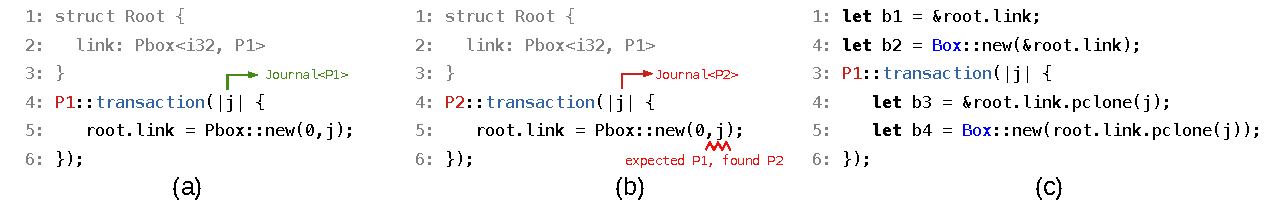
\includegraphics[width=7in]{Figures/links.pdf}
  \end{center}
  \caption{\label{fig:links} {\bf Different Links in \This{}.} (a) Legal assignment to an intra-pool pointer on line 5. (b) Illegal inter-pool pointer assignment; The \csym{Pbox} pointer at line 5 allocates memory from \csym{P2} and attempts to assign in to \csym{root.link} which is a \csym{P1} pointer. (c) A selection of Legal volatile to PM temporary pointers/borrows.}
\end{figure*}

\begin{figure}
  \begin{center}
  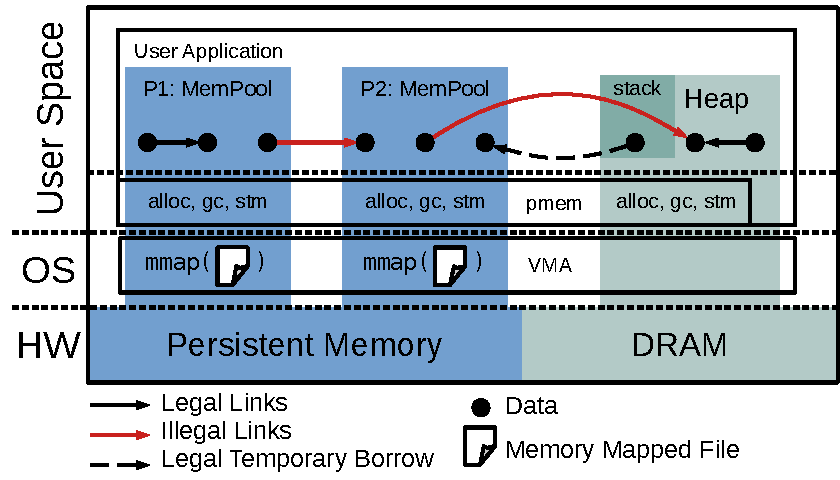
\includegraphics[width=3.2in]{Figures/stack.pdf}
  \end{center}
  \caption{\label{fig:stack} {\bf\this{}ic system stack.} Each \csym{MemPool} is associated with a memory mapped file. It provides memory management and logging interface. \csym{MemPool}s are isolated which means that inter-pool links are illegal. }
\end{figure}
}



% \refsec{sec:ptrs} describes how \This{} implements these constraints in detail. \steve{Do we have a `sec:ptrs' section?}

% \morteza{can we have inline code examples?  just a few lines.  It might be cleaner than using lstlisting.  Or we could have a single figure with (a), (b), (c), etc. for different short examples.}


%Allocation reversibility is required when we have a persistent memory and potentially system crashes to prevent persistent memory leakage. As explained in \refsec{sec:rust}, in Rust, variables drop their owned data when they go out of scope, and the memory occupied by objects is reclaimed when they are no longer in use. However, not only persistent objects may live longer than the program itself, but also they may remain in memory when the process unexpectedly is killed. Therefore, regular memory management mechanisms cannot handle persistent memory leaks.

%Reversible allocation ensures that the memory assigned to an object is not durable until it becomes reachable from the root object, and the transaction is committed. Otherwise, the allocation reverts on failure. The root object is the only persistent object that is accessible after re-opening the pool. \this{} makes sure that the allocation is reversible through a series of considerations. First, it takes a special kind of log for the allocation which indicates that `\textit{this allocation is not persistent}', before returning it. When a crash happens, it reverts the allocation using this log on recovery. Second, the allocator is not publicly visible to the user. Instead, \this{} provides persistent pointer wrappers that closely work with the allocator in background, and are available to the user. \refsec{sec:impl} discusses the details.
\lstDeleteShortInline^

%\section{Implementation}
\label{sec:impl}

Below we describe our implementation of \this{}'s key components.

\subsection{Performance and Scalability}
\label{sec:perf}

The goal of Rust is to provide memory safety without sacrificing performance by implementing a set of rule checking mechanism which is designed to prevent memory related bug. Therefore, the final program is free of the related bugs. \this{} also uses Rust's design. We compare the performance of \this{} and PMDK~\cite{pmdk} in \refsec{sec:results}. However, the performance of \this{} depends on several factors.

\begin{itemize}
    \item Memory management is generic in \this{}. We provide a standard implementation of a Buddy Block allocator which can be used to define new \csym{MemPool}s. However, the programmer may develop a custom allocation mechanism which may or may not be faster than our standard allocator.
    \item Log taking is a costly process. Currently, we use an undo log mechanism which takes log of data only when it is necessary. \this{} is designed in a way that the Rust compiler will warn about unnecessary log taking and transactions. Even if the programmer mistakenly borrow a mutable reference to the object, \this{} does not take log until data is dereferenced mutably (while writing to). \this{} also takes log of data once per transaction.
    \item Log sizes is an important performance issue which it is determined by the programmer. For example, one can wrap a whole array of 1024 elements in a \csym{LogCell} and take log of the array entirely while mutably access it. This might be a good implementation depending on the application. However, if a single element is going to be updated, it is better to have an array of 1024 elements individually wrapped in a separate \csym{LogCell}. Thus, although the programmer does not need to take care of memory-safety, s/he is responsible for the performance.
    \item The underlying device determines how fast can we operate on it. This is out of both \this{}'s and the programmer's control.
    \item The recovery procedure in \this{} is fast as it only need to restore the leftover logs without scanning the entire system.
\end{itemize}

We have designed \this{} to support petabytes of data, and the internal memory usage is a fixed number. \this{} also can be used on any type of storage system as long as a DAX filesystem can run on top of it. The performance of \this{} crate is a factor of the size of transactions and not the size of the device. In case of using a block device rather than a byte addressable persistent memory, \this{} should be configured with a flag that forces it to use \msync{} instead of a write barrier. 


\subsection{Memory Allocation}
\label{sec:mem-alloc}

\This{} uses a persistent buddy allocator that includes features
to provide scalability and support for \this{}'s transactional interface.  Most
of it is implemented in normal Rust, but the low-level allocation code (which
programmers do not interact with directly) is unsafe.

The allocator keeps a free lists for each power-of-two size of memory chunk starting at 8 bytes.  On allocation it searches the list that holds the smallest chunks that could hold the requested space.  If the list is empty, it splits a chunk from the next smallest free list.  The allocator maintains one set of free lists for each core to minimize contention.

The allocator works with the transaction system to ensure leak-free memory allocation.  During a transaction, the allocator logs memory allocation operations internally.  After a crash, the allocator rolls back the operations if the transaction had not committed.  Otherwise, replays the allocations to complete them and make them persistent.  A similar mechanism applies to deallocations.


\ignore{
We
integrate a fast, self-contained, atomic memory allocator in \this{} by
implementing \textit{buddy allocation} algorithm, all packed in \csym{BuddyAlloc} type. It is self-contained because it does not use any resources other than the pool itself to keep its metadata information.  It is also failure-atomic which means that the whole process of allocation/deallocation is reversible in case of a crash. We also make it thread-safe by \steve{providing each core with a separate allocator, and} guarding the operations with a spin-lock \steve{to prevent data race when one core attempts to use another core's qouta due to lack of space}.}

\ignore{\subsubsection{Allocation algorithm.} We implement buddy-block algorithm to provide fast and efficient memory allocation. The allocator consists of 61 sorted linked-lists for free memory blocks of sizes between $2^3$ and $2^{64}$ bytes ($\lst_3..\lst_{64}$). Because we use the first 8 bytes of every free block as a pointer to the next free block, a block cannot be smaller than 8 bytes.
To \textit{allocate} $n$ bytes, we first search $\lst_{\lceil \text{log}~n\rceil}$ for a free block with the size of the smallest power of two that is larger or equal to $n$. If there is no such block, the allocator searches for the next smallest power of two in $\lst_{\lceil \text{log}~n+1\rceil}$ and splits it in two halves. Then, it uses the first one and puts the second one in $\lst_{\lceil \text{log}~n\rceil}$. The allocator recursively reiterates this process on $\lst_i$ where $\lceil \text{log}~n\rceil < i \le \lfloor \text{log}~size \rfloor $ until either it finds a free block or memory exhausts.
To \textit{deallocate} address range of $[a,a+n)$, we should put a free block back to $\lst_{\lceil \text{log}~n\rceil}$. However, if there is a buddy block in the same list, which can be either $[a-n,a)$ or $[a+n,a+2n)$, they merge together to provide a larger free block which is either $[a-n,a+n)$ or $[a,a+2n)$ in $\lst_{\lceil \text{log}~2n\rceil}$. We recursively reiterate the process until no buddy block is found.}

   \ignore{       

\subsubsection{Two-level atomicity.} Since the memory allocation is subject to crashes, we consider a \textit{low-level} atomicity for the metadata consistency, as opposed with the \textit{high-level} atomicity in which the allocation is assumed to be failure-atomic and the reversibility is guaranteed through \csym{DropOnCommit} and \csym{DropOnFailure}. In the low-level atomic section, we log the required updates to the buddy lists in a fixed size auxiliary buffer. At the end of the atomic section, we start draining the buffer and applying the changes to realize the allocations. When a crash happens, we first finish draining the buffer, then, we use the low-level drop logs to revert the operation.
%Note that the low-level drop logs are different from the high-level logs. Low-level logs are limited in quantity and they are used only when a crash happens in the middle of memory allocation/deallocation to protect metadata. The high-level drop logs are unlimited and they are used when a crash happens in a high-level transaction to prevent memory leaks and pointer-related bugs.
\reflst{lst:llatom} shows how the low-level atomicity is used to avail high-level reversibility. At line 3, a new memory block is temporarily allocated in low-level logs. At line 4, we allocate a high-level log for reversibility. Although we record all required changes to the allocator, none of the allocations realizes until the end of the atomic section. If a crash happens, depending on the completeness of the low-level atomic section, we decide to whether realize the allocations, or discard the low-level logs.

\begin{lstlisting}[caption={Atomic allocation},label={lst:llatom}]
fn new<T>(x: T, j: &Journal) -> &mut T {
    Self::atomically(||{
        let p = Self::new_nolog(x);
        Log::drop_on_failure(p, j);
        p
    })
}
\end{lstlisting}
}

Programs cannot invoke the allocator directly.  Instead, they invoke the \csym{new} method of \csym{Pbox<T>}, \csym{Prc<T>}, or \csym{Parc<T>}.  Deallocation occurs when a \csym{PBox} goes out of scope or the reference count for a \csym{Prc} or \csym{Parc} goes to zero.

\ignore{
\subsubsection{Allocation interface.} To protect memory management subsystem from corruption, low-level operations are not available to the user. Instead of that, \this{} provides three persistent pointer type wrappers (i.e. \csym{Pbox<T>}, \csym{Prc<T>}, and \csym{Parc<T>}) that allows dynamic allocation and deallocation through RAII. \steve{These type wrappers have the same properties as Rust's standard pointer wrappers which are described in \refsec{sec:wrapper}, except that they internally manage persistence safety, and they accept a \csym{NVSafe} type for data (\csym{T}) and a pool type \csym{P}}. The constructor methods use the \csym{new} function (\reflst{lst:llatom}) to allocate memory which guarantees reversibility on failure. The destructor method only allocates a \csym{DropOnCommit} log for the data. As they describe themselves, they drop the allocation for data depending on the transaction's status, atomically.
}



\subsubsection{Data Race Prevention}
\label{sec:no-race}

Inherited from Rust, \this{} guarantees an absence of data races. The general form of data race which might happen by aliasing a mutable reference is impossible in Rust. Therefore, the programmer may not send a mutable reference to a thread. However, interior mutability allows threads to mutably borrow data from immutable references. To prevent multiple mutable references in multiple threads, \this{} marks \csym{LogCell} and \csym{LogRefCell} as not being \csym{Send} and \csym{Sync}. However, \csym{Mutex} allows synchronously obtaining a mutable reference to the shared data once at a time, so it is \csym{Send} and \csym{Sync}.

Another undesirable data race may happen while updating the reference counters in \csym{Prc}. To prevent that, \this{} uses atomic counters in \csym{Parc} and disallows \csym{Prc} to be sent or shared between threads. Prevented by trait bounding, the only possible way to have share data of type \csym{T} between multiple threads is to use \csym{Parc<Mutex<T>{>}} (or other arrangements of them).


\subsection{Transactions}
\label{sec:mutex}

\subsubsection{Isolation}

In PM programming, it is not enough to synchronize mutable accesses to data, because releasing the lock after the mutation does not prevent another threads to acquire it, update data, and persist it before the current thread finalizes the transaction (\reffig{fig:mutex}). Additionally, it is possible that the system take double undo logs for the same data, and the the recovery procedure becomes nondeterministic. To prevent that, our \csym{Mutex} locks data throughout the whole transaction and allows re-entrance from the same thread to prevent deadlock.

\begin{figure}%[!ht]
    \begin{center}
    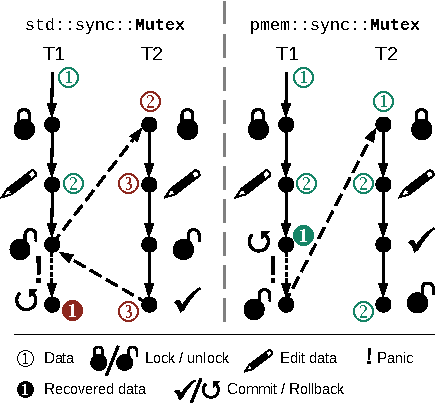
\includegraphics[width=3in]{Figures/tramutex.pdf}
    \end{center}
    \caption{\label{fig:mutex} {\bf Volatile and Persistent Mutex.} As shown on the left, standard \csym{Mutex} may lead to an inconsistent state by rolling back the incomplete transaction after letting data be updated and committed in another thread. On the right, persistent \csym{Mutex} locks data throughout the transaction's lifetime until it finishes to guarantee data consistency.}
\end{figure}

\subsubsection{Unstable Features}

Rust has a sophisticated system for allowing programmers to opt-in to
experimental language features.  Many (but not all) of the experimental
features eventually find their way into the official language.  Our
implementation of \this{} relies on several of these experimental features, but
none of them are fundamental to \this{}'s design: \csym{untagged\_unions}, \csym{specialization}, \csym{optin\_builtin\_traits}, \csym{llvm\_asm (for c lflush\_opt and low level stuff)}, \csym{core\_intrinsics}, \csym{negative\_impls}, \csym{const\_generic\_impls\_guard}, and \csym{const\_generics}.


%% Memory leaks and related pointer bugs are common problems in programming
%% systems when a piece of memory becomes unreachable or unavailable. We address
%% these issues by implementing persistent pointer type wrappers that protect data
%% and the memory management subsystem. \reftab{tab:types} lists the three
%% persistent pointer wrappers. These pointer wrappers share four characteristics
%% for safety: 1) their constructors}/destructors are transactional in order to
%% avoid memory leaks; 2) they do not provide interior mutability to make sure
%% data does not change in crases; 3) additional to the data type, they require a
%% pool type as a part of the wrapper to enforce pool isolation, and 4) they
%% cannot move out of an atomic section unless they become reachable from the root
%% object.

% \subsection{Persistent Pointer Type Wrappers}
% \label{sec:wrappers}

% Persistent objects and volatile objects do not have much differences other than their memory locations. A volatile object reside in the heap and is referenced by a volatile pointer, and likewise, a persistent object resides in the PM and is referenced by a persistent pointers. Since Rust does not provide persistent pointers, \this{} expands Rust's design by providing the persistent version of Rust's standard pointer type wrappers (\refsec{sec:wrapper}) that protect data from system crashes: \csym{Pbox<T,P>}, \csym{Prc<T,P>}, and \csym{Parc<T,P>}. These type wrappers have the same properties as Rust's standard pointer wrappers which are described in \refsec{sec:wrapper}, except that they internally manage persistence safety, and they accept a \csym{NVSafe} type for data (\csym{T}) and a pool type \csym{P}. 

% \subsubsection{Concurrent Access.} Multiple threads may want to allocate from the PM or release memory. Since the PM is a shared resource, it should be protected against data race. We dedicate an individual allocator over a separate memory chunk to each core in order to mitigate the contention. To allow borrowing memory from another chunk on memory exhaustion, each allocator leverages a fast spin lock. Note that the lock is not effective on local allocations.

%% \subsection{Pointer Safety}
%% \label{sec:pointers}

%% The referential integrity invariant means that all pointers in the course of program execution, point to a valid data. This can be provided by enforcing a set of rules that provably prevent undesirable pointer-related bugs. PM programming shares many of this kind of bugs with heap-based programming model. Fortunately, Rust provides pointer safety for that class of bugs. Inspired by Rust's design, we extend its pointer safety to our persistent smart pointers.

%% \subsubsection{Pointer-Data Coexistence}
%% \label{sec:no-dangl}

%% Dangling pointers appear when the lifetime of a pointer is longer than the lifetime of data it points to. Similarly, memory leaks happen when a pointer dies while its data is still alive and unreachable. Rust prevents the former situation by applying drop chain through enforcing RAII. The latter situation is also not possible in Rust since the deallocation of data is controlled by the owner pointer. However, it may happen in PM programming due to write reordering or a crash in the middle of the drop chain. Our persistent pointer types have the same dropping mechanism as the standard smart pointers, except that they use our atomic, leak-free allocator and their counters (if any) are failure-atomic. By enforcing all changes to a pointer (i.e. construction, destruction, and reassignment) to be transactional, holding pointer-data coexistence invariant is guaranteed.

%% \subsubsection{Non-existance of Wild Pointers}
%% \label{sec:no-wild}

%% The smart pointers in Rust own data, which means that they exclusively control over the data creation and destruction. This feature eliminates the possibility of appearing wild pointers, as the pointer allocates its own data. \This{} guarantees non-existence of wild pointers in a similar way. That is the creation of data happens before the creation of owner pointer. Our allocator guarantees the atomicity of the data allocation by packing the data and a drop log in a single atomic allocation. In case of a failure, either both data and its drop log exist, or none of them do. Therefore, the high-level transaction can revert the allocation on recovery using the drop log, if it exists.

%% \subsubsection{Transactional RAII.} In \this, dynamic allocation is available through persistent pointer wrapper constructors which requires a \csym{Journal} object to perform which trivially enforces their invocation to be inside a transaction. To make the destruction transactional too, we should prevent their invocation from outside a transaction which is non-trivial. This is because of Rust's reliance on RAII which may lead to memory deallocation on data assignments. \this{} promises transactional deallocation by enforcing two invariants: 1) no mutation outside transaction, and 2) there should be a path from the root object to this allocation. The former prevents deallocation due to reassignment, and the latter prevents deallocation due to zero references. \reflst{lst:alloc} shows how allocated object can move out of a transaction. The old value of \csym{root} drops at line 5, and the recently allocated object `\csym{new}' replaces it, all happening inside the transaction.

%% \begin{lstlisting}[caption={Transactional data construction/destruction},label={lst:alloc}]
%% type Root = LogCell<Pbox<i32,P>,P>;
%% let (root,p) = P::open::<Root>("1.pool",0);
%% P::transaction(move |j|{
%%     let new = Pbox::new(1, j);
%%     root.set(new, j);
%% }).unwrap();
%% \end{lstlisting}

%% \subsubsection{Loggable interior mutability.} To prevent data loss, we should make sure that the mutations are recoverable. \refsec{sec:over:log} explains recoverable mutation and why it is important in PM programming. To achieve that, the persistent pointer wrappers do not allow mutable dereferencing. Once initialized in a transaction, interior data cannot change. However, this vastly limits the programmability. As explained in \refsec{sec:over:log}, \this{} provides crash-safe interior mutability though a set of memory cell types (the last two rows of \reftab{tab:types}). In contrast with the persistent pointer types, memory cell types wrap around the actual data. They provide special interface for interior mutability that assures the recoverability by taking undo logs before mutation. For example, in \reflst{lst:alloc}, \csym{root} is a memory cell of type \csym{LogCell} that takes a \csym{DataLog} before mutation at line 5.



%% \ignore{
%%     \subsection{Thread-safe pointers}
%%     \label{sec:thrd-safe}
    
%%     \steve{\csym{Prc} and \csym{Parc} both allow sharing data between multiple owners, and manage memory allocation using reference counting. However, when they are shared between threads, data racing might happen while updating the counters. Therefore, since only \csym{Parc} uses atomic counters, we mark it as \csym{Sync} and \csym{Send} to allow being sent and shared by multiple threads. Remember that both \csym{Prc} and \csym{Parc} use failure-atomic counters which are logged before mutation, but \csym{Parc} additionally uses thread-safe atomic counters.}
%% }



% \subsection{Failure Atomicity}
% \label{sec:atomic}

% \reffig{fig:trans} shows the anatomy of a transaction that provides failure atomicity for updating persistent objects. The low-level operations are integrated into \cfunc{transaction} and \cfunc{borrow\_mut}. The write order is preserved by persisting the logs (using \clflush{}, or \clflushopt{}/\clwb{} followed by a \sfence{}) before mutation. We apply source-data swap~\cite{log-nvmm} while taking a log to save one costly persist barrier after updating data. Depending on the result of executing the transaction's lambda, \this{} commits the changes on success, or rolls back them on failure. Then removes the logs from the journal. If a crash happens, the recovery procedure uses the persisted logs to restore the system back to its state before the transaction. The lambda can capture variables bounded by \csym{TxInSafe}, and may return values marked as \csym{TxOutSafe}. Exclusive availability of a reference to the journal object \csym{j} inside a transaction constraints functions taking it as an argument to be enclosed by a transaction.

% To enforce {\it Ordered Writes} and {\it Recoverable Mutation} invariants, \this{} provides atomic sections through software transactional memory (STM) technique and Rust's borrowing mechanism. Working together, \this{} prevents unrecoverable modification to data by taking an undo log before mutating data and preserving persist order of the logs in an atomic section. \reffig{fig:trans} shows a failure-atomic transaction in which a persistent data changes. As shown in this figure, write ordering preservation is hidden. Since journals are created inside a transaction, functions that take a journal as an argument, such as \csym{borrow\_mut} can only be used inside \csym{transaction}. Also, since the mutable borrow is created in the atomic section, Rust's lifetime checker prevents sending it out of the atomic section which may have consequences otherwise. \this{} is designed in a way that the programmer writes the code while holding the invariants without being aware of them. 


% \subsection{Interior Mutabilty}
% \label{sec:mut}

% Interior mutability means that a variable of a wrapper type allows mutable access to its inner value while the outer wrapper is not mutably borrowed. For example, Rust has a type wrapper called \csym{UnsafeCell<T>} which has a method with the following signature: \csym{UnsafeCell<T>::get(\&self) -> *mut T}. Although the \csym{get} function does not require the variable to be mutable, it returns a mutable raw pointer to its inner data of type \csym{T}. This is unsafe to provide interior mutability for persistent objects unless we make sure that data is logged. By definition, \csym{Pbox}, \csym{Prc}, and \csym{Parc} do not provide interior mutability. In \this{}, there are three other type wrappers that safely expose a mutable reference to the protected data: \csym{LogCell}, \csym{Mutex}, \csym{RwLock}, and \csym{Tramutex}. \csym{LogCell} and \csym{LogRefCell} provide interior mutability via functions \csym{set()} and \csym{borrow\_mut()}, respectively, which take a reference to a \csym{Journal}. Its argument forces the programmer to wrap the code in a transaction. \csym{Mutex}, \csym{RwLock}, and \csym{Tramutex} basically have the same mechanism, but they are used for serialization in multi-thread programming. In \reflst{lst:mut}, \csym{list} is of type \csym{Prc<LogRefCell<List,P>,P>} that wraps a pointer to a \csym{List} object inside a \csym{LogRefCell}. In this case, the pointer can only be read, but the whole wrapped persistent pointer can be mutably borrowed as it is in line 9.

% \begin{lstlisting}[caption={Mutably borrowing a persistent object},label={lst:mut}]
% type Ptr = 
%     MaybeNull<Prc<LogRefCell<Node,P>,P{>}>;
% struct Node { val: i32, next: Ptr }
% struct List { tail: Ptr, length: i32 }
% fn add_element(
%     list: &Prc<LogRefCell<List,P>,P>, 
%     val: i32) {
%     P::transaction(move |j|{
%         let mut list = list.borrow_mut(j);
%         list.tail = Valid(Prc::new(
%             LogRefCell::new(Node{
%                 val, next: Null
%             },j),j));
%         list.length += 1;
%     }).expect("Unsuccessful");
% }
% \end{lstlisting}

% The common use of these types is for wrapping the inner value of these pointer wrappers. \reflst{lst:mut} represents a snippet of code that attempts to add a new element to a linked list residing the \csym{P}. The type \csym{List} consists of an optional persistent pointer to the tail of the list, and the length of the list. A \csym{Journal} object for \csym{P} is created at line 8 when we open a transaction. Line 9 takes an undo log of the list data structure. The log is not for entire list, however, it only keeps the old value of the tail pointer and the length of the list. After taking a log, \csym{borrow\_mut()} returns a mutable reference to the list. Any changes being made from this point on to \csym{list} is recoverable. The key point of this implementation is that there is no unsafe way to make changes. Unlike other persistent libraries in which the programmer should call some kind of logging function at the beginning of the transaction (e.g. PMDK~\cite{pmdk}), in \this{} the log taking process is hidden behind Rust's borrowing mechanism. 


% \subsection{Software Transactional Memory}
% \label{sec:stm}

% Software Transactional Memory (STM) is a common practice to control access to the shared data and protect it from system failure in the persistence context. \this{} also is featured with STM to satisfy the invariants described in \refsec{sec:atomic}. Transactions in \this{} have the following properties.

% \begin{itemize}
%     \item \textit{Log Structured}: Opening a transaction creates a \csym{Journal} object, and this is the only way to obtain a reference to a journal. Therefore, when a function takes a journal object as an argument, it basically means that it can be called only from a transaction.
    
%     \item \textit{Thread/Pool Separated}: Each thread can open one transaction per memory pool. Calling transaction function multiple times is allowed but they all refer to the same \csym{Journal} object.
    
%     \item \textit{Matryoshka Principle}: Nested transactions are allowed, but they are ineffective in committing changes. However, if a panic happens, the exception is propagated up to the top transaction and abort all of them. This allows functions to have their own transactions to make sure that their operations are atomic-safe.
    
%     \item \textit{Returning Results}: Transactions can return data of any type with a constraint that it should implement \csym{TransactionOutSafe} trait. None of the persistent pointer wrappers implements this trait. It means that a persistent object cannot live longer than the transaction unless it becomes reachable by the root object.
    
%     \item \textit{Unique Pool Access}: Since transactions belong to pools, only one type of journal is available within a transaction. This means that allocation from multiple pools is not possible inside one transaction (\reflst{lst:cross}). However, nested transaction from different pools is allowed and safe.
% \end{itemize}

% We applied these restrictions to assure that none of the safety invariants is possibly violated. For more clarification, we first explain our journaling mechanism, and then describe how the STM and journaling mechanisms guarantee the satisfiability of the invariants.

% \subsubsection{Journaling} To track the uncommitted changes to the persistent memory, we should durably record all versions of the data in persistent memory. We use undo-logging which means that \this{} writes the old version of data into a data structure called \csym{Journal} right before making changes to the original data. This process happens once per transaction for every data that is going to be modified.

% There are five types of logs:

% \begin{enumerate}
%     \item \csym{DataLog} is the regular log as described above for undo-logging.
%     \item \csym{DropOnFailure} is created while allocating of new data to be used when a power failure happens for reclaiming the allocation as explained in \refsec{sec:mem-alloc}.
%     \item \csym{DropOnCommit} is made while freeing a persistent object. The log will be used to resurrect the object when the transaction was unsuccessful, or system fails.
%     \item \csym{UnlockOnFailure} is used when a lock is acquired and system fails. To release the locks after recovery, \this{} uses logs of this kind to find them (used in \csym{Mutex} and \csym{RwLock}).
%     \item \csym{UnlockOnCommit} is used to release a lock after committing/rolling back a transaction. It also releases the lock on system failure (used in \csym{Tramutex}).
% \end{enumerate}

% According to our rollback journal model, we should make sure that the logs are persistent before modifying data. Therefore, \this{} issues  \clflush{}/\clflushopt{}/\clwb{} and \sfence{} for every corresponding cache line belonging to the log. By doing this, \this{} makes sure that the subsequent writes are safe (it satisfies `Memory Ordering' invariant).

% \begin{figure}%[!ht]
%     \begin{center}
%     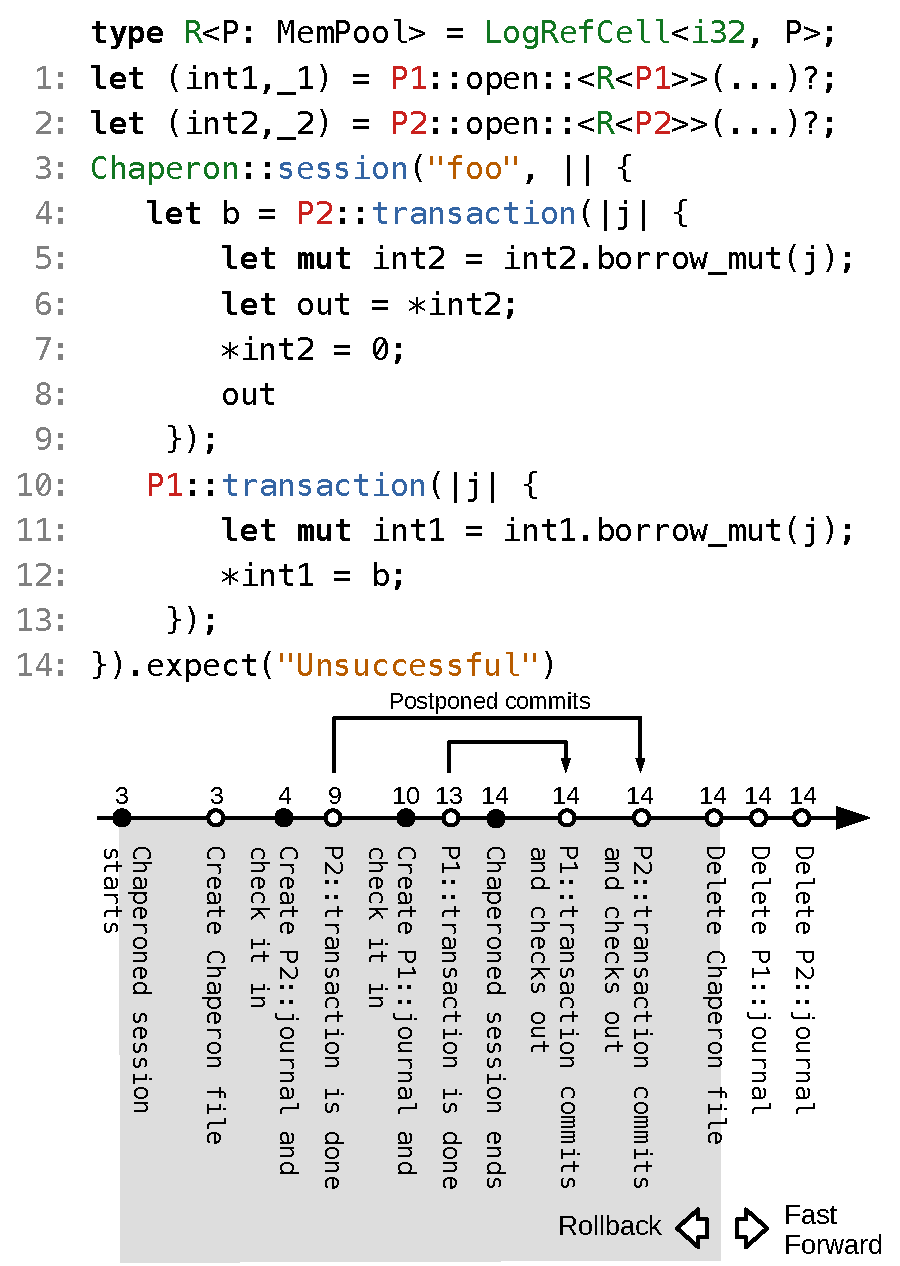
\includegraphics[width=3.2in]{Figures/attach.pdf}
%     \end{center}
%     \caption{\label{fig:cross} {\bf Cross-Pool Transaction.} \csym{Chaperon::session()} provides an atomic section for multiple pools to update persistent objects. The failure atomicity is provided by a separate data structure that monitors all transactions.}
% \end{figure}

% \subsection{Cross Pool Pointers}
% \label{sec:cross-pool}

% \steve{partialy redundant (sec 4.3: Pointers to Persistent Data)}

% To provide persistent memory access, we defined a special Rust trait which is called `\csym{MemPool}'. It provides all required methods for memory management. The key feature of this trait is that none of its methods has access to \csym{self}. In other words, it requires all management information (e.g. flags, size, available space, etc.) to be static. Therefore, \csym{MemPool}s are actually different types rather than being different instances of a single type. This actually helps us to reuse Rust's strong type checking rules to make sure that pointers cannot refer to different pools.

% The provided pointer wrappers should be given a type for the protected data, as well as a type as the belonging memory pool. Now, it won't be possible for a pointer to point to data allocated in another pool. However, to be able to work these pointers, we need to obtain the protected data from the function's stack memory. Therefore, we considered a special case that allows temporarily lending the protected data to references residing in the heap. This is safe because if a crash happens, volatile pointers wont exist to become wild pointers, and data has already an owner in the persistent region.



% \subsection{Reference Counting}
% \label{sec:ref-cnt}

% % Reference counting is a programming technique for automatically deallocating shared resources when they have no more references. 
% \csym{Rc} and \csym{Arc} in standard rust use reference counting to manage the allocation under RAII. References can be either strong or weak. A strong reference to data guarantees the validity of the referent while a weak reference my be dangling. When the number of strong references becomes zero, the allocation for shared value should drop. If the number weak references is also zero, the counters also drop. Weak pointers are used for cyclic referencing and they do not count for value deallocation.

% \this{} also implements reference counting technique in a vey careful way: the counters should be recoverable. This makes the implementation \csym{Prc} and \csym{Parc} much more complicated. To instantiate another owner to the shared data in these types, a \csym{clone} function is provided to conform Rust's design with a small deference: in \this{}, \csym{clone} takes a journal to provide recoverability. This means that these types can be cloned only inside a transaction. This is because their reference counters are crash-safe.

% \begin{lstlisting}[caption={Reference counting example for (A) \csym{p1: Rc<T>}, and (B) \csym{p2: Prc<T>}},label={lst:ref-cnt}]
% // (A) Standard Rc
% // Creating another reference to data
% // and incrementing its strong counter
% let other = p1.clone();

% // (B) Persistent Prc
% transaction(|j|{
%     // Taking a log of the counters and
%     // performing Rc's similar process
%     let other = p2.clone(j);
% });
% \end{lstlisting}

% \reflst{lst:ref-cnt} compares the process of incrementing strong counter in standard Rust and \this{}. When we have a log for the counters, we can confidently increase it by instantiating another owner for the shared object. In case of a crash inside the transaction, the allocation for \csym{other} drops during the recovery process. This means that the number of strong references to the resource should be subtracted by one. However, we do not have access to the counter during the recovery because we cannot maintain type system information in the persistent memory (types are zero sized). But, there is no problem here because we already took a log of the counter when it was intact. A simple rollback operation makes the counter consistent again. The same process is taken for weak counters.

% \subsection{Concurrency}
% \label{sec:parallel}

% As explained in \steve{4.9.3 Memory Allocation}, \this{} manages concurrent access to the PM via concurrent allocators, and \refsec{sec:thrd-safe} explains how \csym{Parc} protects shared resource from data racing. \csym{Pbox} is also thread-safe because it is the only owner of the value. When it moves to a thread, other threads cannot access its data. Here, we discuss the challenges with updating shared data in a \csym{Parc}, and how \this{} addresses them.

% Data race is the major problem in concurrent and parallel programming. Rust perfectly manges to handle data race problem by its ownership and type systems. Inherited from Rust, \this{} also handles concurrency issues. Rust provides two auto traits of \csym{Send} and \csym{Sync} to determine that a type is safe to be sent across thread boundaries, and be shared between multiple threads, respectively. To determine which type is thread-safe and which is not, we used Rust's builtin traits of \csym{Send} and \csym{Sync}.

%  \csym{Prc} and \csym{Parc} allow multiple ownership of data and manage memory through reference counting. However, \csym{Prc} is not thread-safe because the reference counters are not atomic in order to provide high-performance.

% \subsubsection{Interior mutability.} It is critical to differentiate between \csym{LogCell} and \csym{Mutex}/\csym{RwLock}, because other than recoverability, there should be some sort of locks to protect data from data race in parallel programming. Therefore, complying Rust standard model, \csym{LogCell} is marked as thread-unsafe while the other two are thread-safe. % \reflst{lst:thread} demonstrates an example of using a crash-consistent multi-thread application.

% \subsubsection{Poisoning.} When a thread raises an exception, other threads may still think that the shared data is legitimate. To prevent that, \csym{Mutex} and \csym{RwLock} leverage a poisoning mechanism to notify other threads that data is corrupted in subsequent accesses. Therefore, the result of locking is either a guard object that allows accessing data through dereferencing, or an error object when the previous locking thread panicked. The error object also wraps a guard object to allow working with data after handling the exception.


% \subsubsection{Transaction-scope serializrion.} Although \csym{Mutex} and \csym{RwLock} safely serialize access to shared data in the locking scope, the consistency of data cannot be guaranteed when the scope is smaller than the transaction scope. To shed light on this problem, \reffig{fig:mutex} graphically explains the inconsistency problem with \csym{Mutex}. As shown in this figure, \csym{Mutex} protects shared accesses to data while it cannot protect it when the crash happens between unlocking data and committing the transaction. As a result, data will be recovered to a wrong value. To avoid this situation, \this{} considers \csym{Mutex} and \csym{RwLock} unsafe (only for non-critical data), and offers \csym{Tramutex} which is a transaction-wide thread-associated lock. Once the lock is acquired, other threads cannot access data until the transaction is done. To avoid deadlock, the subsequent locks in the same transaction are non-blocking.

% \subsubsection{Mutex vs. Tramutex.} The main difference between \csym{Mutex} and \csym{Tramutex} is their scopes which is explained above. In addition to their different scopes, they offer different performance characteristics. \csym{Tramutex} serializes the whole transaction which destroys the performance gain of multi-threading when the thread only contains a single transaction (e.g. \reffig{fig:mutex}). We recommend using multiple transactions with \csym{Tramutex} inside a thread, for critical data, and use \csym{Mutex}/\csym{RwLock} for less critical data. To make sure that the user is aware of \csym{Mutex}'s problem, the \csym{lock} method is marked as unsafe.


% \subsection{Limitations}
% \label{sec:limit}

% Although \this{} provides fast, safe, and easy-to-use interface to the PM, it has a few number of limitations:

% \begin{enumerate}
%     \item The number of memory pools should be statically known at the compile time. This limits the flexibility of having arbitrarily number pools. We implemented an indexed pool version to lift this limitation at the cost of a performance overhead for dynamically checking pool-isolation rule.
%     \item Rust is a young programming language and it has a steep learning curve.
%     \item \steve{please add more if you find more}
% \end{enumerate}

% We believe that these limitation does not mitigate the value of high-performance and safety features of \this{}, even though we are actively improving the library fo the public use.


\ignore{There are no Flaws.

Flaws are -- 1.  Allocated and not reachable or 2. reachable and not allocated
Flawless = (allocated and reachable) or (not allocated and not reachable)

Assume P is flawless.  Prove that nothing can occur that would create a flaw.

We only need to consider what happens in a transaction as a whole, because the
allocation operations for a transaction either all occur or do not occur.

1.  x is Allocated and reachable
    a.  at the end of a transaction, x becomes not allocated but still reachable
        i.  not possible by reference counting (Prc) and raii (pbox)
    b.  at the end of the transaction, x becomes unreachable
        i.  **** there was path from the root to x, and it was broken.  how?  pointer assignment.  Why cannot that happen?  What about an interrupted cascading drop?
            A. the allocation of x does not drop until the transaction commits the corresponding DropOnCommit log
            B. before deallocating x, and while dropping x inside the transaction body, we recursively call to the drop functions of x's decendents and create a DropOnCommit log for every single of them
            C. transactions have a two-phase finalization process: commit/rollback and clear.
                1-a. when transaction finishes without panic or crash, it starts committing the logs. If crash happens, we continue committing the logs on recovery (deallocating DropOnCommit).
                1-b. when transaction is broken or crash, it starts rolling back. If crash happens, it continues rolling back on recovery. It reverst the reassignment and discards the allocation (DropOnFailure).
                2. when all logs are committed/rolled back, then it frees the logs. If a crash happens, it continues freeing the logs on recovery.
            D. due to B and C, the path from root to x never gets broken
            E. The reference counters are recoverable, so, it gets back to its consistent state on recovery
            F. Local y may refer to x and increaments its ref counter, but it will drop at the end of transaction because it cannot go out of it, and so, decreases x's ref counter back.
    c.  x becomes unreachable and unallocated
    	i. ok! still flawless
	
2.  x is not allocated and not reachable
    a.  at the end of a transaction, x becomes allocated (but not reachable)
        i.  **** x could be assigned to many kinds of pointers (pbox, prc, parc, local to tx, global, captured by tx, etc..  Why are each of them either safe or impossible?
            A. RAII makes x drop itself if it is not references by an object which can go out of scope
            B. If a crash causes its unreachablility, the allocation drops on recovery by DropOnFailure
            C. No mutable reference or pointers (box, rc, arc, pbox, prc, parc, local to tx's parent, &mut T, *mut T) can cross the transaction boundaries, so they be captured by transaction and thus, cannot refer to x
            D. if x is a persistent pointer, it cannot go out of transaction too, so, the referencing should happen inside transaction to keep x alive
            E. global mutable objects are naturally unsafe in Rust
    b.  at the end of a transaction, x becomes reachable (but not allocated)
        i.  basic pointer safety.
            A. not possible becuase the allocation process is hidden, and happens before assignments (or referencing)
    c.  x becomes reachable and allocated
    	i. ok!  Still flawless.


Then do induction starting at an empty pool where everything is unreachable and unallocated, except the root.


int * foo;  // thing that holds the name of a piece of memory.

foo = \malloc{} (); // the thing that \malloc{} returns is the name of a piece of memory.

foo: Box<Cell<int{>}>


bar: PBox<int>
bar: PBox<PCell<int{>}>

foo = 0

let bar: PBox<int> == const int *; // acts like `const int'
let mut bar: PBox<int> == int *; // acts like `int'

let bar: PBox<PCell<int{>}> == int *; // acts like `int'
let mut bar: PBox<PCell<int{>}> == int *; // acts like `int', too

let bar: int == const int
let mut bar: int == int
let bar: PCell<int> == int
}

%auto-ignore

\section{Evaluation}
\label{sec:results}

We evaluate \this{} along three axes: its success in statically enforcing PM
safety properties, its ease of use, and its performance.

\subsection{Static Checking}

\This{} aims to make the programmer's life easier by statically enforcing PM safety at compile time rather than relying on dynamic checks and testing to identify bugs.
To measure its success in this regard, we
compare it with other PMEM programming systems.

\reftab{tab:libs} summarizes how \this{} and other PM libraries detect violations of
\this{}'s six design goals.  In the table, ``S'' (for ``Static'') means that the compiler
either enforces the invariant automatically (e.g., by generating safe code) or detects any violations and
reports them, ``D'' (``Dynamic'') means that the system will identify the problem at
runtime and exit appropriately, % \steve{not always exits: V-to-NV returns a Result which without panic. If you unwrap the Result, then it panics.}
and ``M'' (``Manual'') means that the system does not detect
violations, so they will manifest as a crash, data corruption, or
other error.  For \nameref{goal:no-memory-leaks}, ``GC'' means the system
provides garbage collection.

The table shows that \this{} enforces almost all its invariants at compile
time, compared to the relatively few compile-time checks other systems provide.

In some cases, this difference represents a design trade-off.  For instance,
NVM Direct explicitly supports unlogged stores as performance optimization.
Likewise, four of the systems allow unsynchronized access which is faster but
less safe.  A \this{} programmer could use similar techniques to improve
performance with \csym{unsafe}.

\begin{table}
  \footnotesize
  \center
  \begin{tabular}{|r||c|c||c|c|}
    \hline
    App & Rust & \This{} & C++ & PMDK \\ \hline\hline
    Linked List & 192&+19 (9.9\%) & 146&+45 (30.8\%)  \\ \hline
    Binary tree & 256&+12 (4.7\%) & 208&+41 (19.7\%) \\ \hline
    HashMap     & 165&+10 (6.1\%)  & 137&+42 (30.7\%) \\ \hline
  \end{tabular}
  \caption{Adding persistence to data structures with \this{} requires fewer
    changes (measured in lines of code) than PMDK.}
  \label{tab:loc}
\end{table}

\subsection{Ease of Use}
\label{sec:ease}

A key goal of \this{} is to make writing safe persistent memory programs
easier.  Qualitatively, we would expect that the stronger static guarantees
that \this{} provides should lead to less debugging.  This is especially
valuable since many of the bugs that \this{} protects against would manifest
during a failure, making them more difficult to test.  Our experience using
\this{} bears this out: once code compiles, it works reliably.  
Getting the code to compile can take a while.

\ignore{
Achieving this is a balancing act: On the one hand, \this{} provides
must stronger safety guarantees that existing PMEM libraries.  This should
reduce the number of bugs and vastly increase programmer confidence that their
code is reliable and correct.  Rust's popularity in the system programming
world demonstrates the value of this approach.

On the other hand, \this{} requires programmers to use Rust, a language that
presents a daunting learning curve and, if you are a C or C++ programmer, the
challenges of cross-language integration.

Consider how this trade-off might play out for an experienced C or C++
programmer who wants to write their first PMEM program.  They could pickup
PMDK~\cite{pmdk} and create persistent data structure relatively quickly, but
they would (or should) have only modest confidence that the structure would
crash consistent and thread safe.  It is likely that their first attempt missed
important corner cases.  With practice, debugging, and careful thought, they
would eventually fix the problems and deliver a working, reliable structure.

Alternately, they could learn Rust and then use \this{} to build the same data
structure.  They would likely find that Rust presents a significant and
sometimes frustrating learning curve.  The pay off is that there are no
segmentation faults and, quite often, if the code compiles, it works.

Adding \this{} presents additional typing complexity and more fighting with the
compiler.  However, once the code compile, it is likely to work, and the
guarantees that \this{} provides provide great confidence that the PM-specific
aspects of the code are correct as well.  This is especially valuable since
bugs in these aspects of the program only manifest during recovery, making them
hard to test.
}
%% Adding \this{} presents additional typing complexity.  Getting
%% the code to compile resembled a series of type checking puzzles.  They were
%% challenging -- perhaps just as hard as carefully checking PMEM code -- but
%% relying on the type checker for correctness removed the anxiety of wondering
%% whether a corner case had been missed.  Again, once the code compile, it
%% generally worked.  Further, because of the guarantees that \this{} provides,
%% the programmer could be confident that the PM-specific aspects of the code were
%% correct as well.  This is especially valuable since bugs in these aspects of
%% the program only manifest during recovery, making them hard to test.


Quantitatively, we can measure programing effort by lines of code needed to add
persistence to a conventional program.  We implemented three data structures in
C++ and Rust and then added persistence using PMDK and \this{}. \reftab{tab:loc} shows
that \this{} required adding fewer lines in both relative and absolute terms.


\ignore{This task is challenging and time consuming.  However, since
\this{} checks many key properties statically, once the code compiles they can
have much higher confidence its crash consistency and thread safety.


While we have not performed a formal user study, the authors' experience with
\this{} provide some perspective on its strengths.  One of the authors (an
experienced C/C++ and PM programmer) had not used Rust.  Over the course of a
week or so they learned Rust and then \this{} by building simple volatile and
then persistent data structures.

The authors' experience using \this{} followed 

\This{} aims to make persistent programming easier for Rust programmers by
making it more difficult to write buggy code.  It also aims to match common
Rust programming conventions, so that

Ease of use is the key advantage of \this{}. Persistent libraries are competing
each other over this metric to provide safe programming environment without
requiring the programmer to be an expert in persistent
programming~\cite{pmdk,nvheaps,atlas,javapersistence}.  Using Rust's standard
programming style, we implement \this{} in an idiomatic and familiar way to
make its usage as simple as possible. For instance, the smart pointers in
\this{} act similar to their volatile cousins.  Additionally, shifting
the persistence bugs to the compile time allows debugging at almost zero cost.

}

% To grasp a sense of differentiation between standard programming in Rust and persistent programming with \this{}, \reflst{lst:reimpl} re-implements the same function in \reflst{lst:mut} in volatile memory.

% \begin{lstlisting}[caption={Reimplementation of \reflst{lst:mut} using std crate},label={lst:reimpl}]
% type Ptr = 
%     Option<Rc<RefCell<Node> > >;
% struct Node { val: i32, next: Ptr }
% struct List { tail: Ptr, length: i32 }
% fn add_element(
%     list: &Rc<RefCell<List> >, 
%     val: i32) {
%     panic::catch_unwind(
%     AssertUnwindSafe(move ||{
%         let mut list = list.borrow_mut();
%         list.tail = Some(Rc::new(
%             RefCell::new(Node{
%                 val, next: Null
%             })));
%         list.length += 1;
%     })).expect("Unsuccessful");
% }
% \end{lstlisting}

% As shown above, except the transaction block which is replaced with a \csym{catch\_unwind()}\footnote{\csym{catch\_unwind()} can be seen as a try-catch block which catches the exception arisen inside the closure.} section and \csym{Journal} object passing, everything else is exactly similar to standard Rust programming while using \csym{Rc<RefCell<T>{>}} instead of \csym{Prc<LogRefCell<T,P>,P>}. This shows how idiomatic \this{} would be for Rust programmers with minimal knowledge of persistent programming. Note that, because there is no rollback mechanism in standard Rust for volatile objects, interior mutability is not allowed in \csym{catch\_unwind} section. Therefore, the programmer takes the risk of undesirable changes by asserting that the closure does not panic. However, Rust recommends not having an unwind catching section with mutable references for memory safety.


\subsection{Evaluation Platform}
\label{sec:res:platform}

Our test platform has dual 24-core Cascade Lake processors.  The CPUs are
engineering samples with specs similar to the Xeon Platinum 8160.  In total, the
system has 384~GB (2 socket × 6 channel × 32~GB/DIMM) of DRAM, and 3~TB (2
socket × 6 channel × 256~GB/DIMM) of Intel Optane DC DIMMs.  Our machine runs Fedora 27 with
Linux kernel version 4.13.0.

\This{} uses some unstable features of Rust, so we use Rust Nightly version
1.51.0 built with `release' profile.  We compared \this{} with PMDK 1.8, Atlas, Mnemosyne built
with `-O2'. All of them use `\clflushopt' for durability without using non-temporal store. The go compiler applies optimizations to go-pmem by default. We use \extfsDAX{} to mount the persistent memory and create the
pool files.

\ignore{\subsection{Testing}
\label{sec:res:qoality}

For QoS, we focus on the crash consistency of data, and there are no metrics to show that other than the quality of being \textit{correct} or \textit{incorrect}. One single \textit{incorrect} situation infers the low quality of the design. \this{} is verified through a series of intensive workload with the presence of possible thread failure. Note that we cannot emulate real power failure since it was not possible to physically unplug the server. Therefore, the write ordering remains untested, while the logging system is verified through manually killing the process, rerunning it, and comparing the results.

\subsubsection{Methodology}
\label{sec:res:qoal:method}

In this experiment, we developed a set of inductive workloads producing progressive results: the output of the process at time $t+1$ depends on the output of the process at time $t$. To fairly test the correctness, a separate process generates \csym{SIGKILL} randomly and kills the running process. Thus, the possibility of crashing is the same at every point of execution. A crash may happen while working with data, taking log, allocating memory, etc. The final results are compared with the normal execution of the program.

% \begin{table}
% \center
% \small
% \caption{Crash consistency workloads}
% \label{tab:qoal:wrkld}
% \begin{tabular}{|p{0.5in}|p{2.5in}|}
%     \hline
%     FFT {\scriptsize (Single-Thread)} & Calculating FFT of a signal of 1000 samples \\ \hline
%     Fibo {\scriptsize (Multi-Pool)} & Calculating the 1000th item of the Fibonacci series. It keeps the last two numbers in two different pools. A chaperoned session is used to atomically update both numbers. \\ \hline
%     Grep {\scriptsize (Multi-Thread)} & MapReduce implementation of a word counter program that finds the frequency of all words in a list of files. Two threads read from file and push string lines with at-least 1024 characters in a shared stack. Another 16 threads pop from the stack, count the words, and update a shared \csym{HashMap} mapping words to their frequency in three separate transactions.  \\ \hline
% \end{tabular}
% \end{table}
}

\ignore{\subsubsection{Workloads}
\label{sec:res:qoal:workload}

% \reftab{tab:qoal:wrkld} shows the three micro-benchmarks we used to verify single-thread thread programs, chaperoned multi-pool programs, and multi-thread persistent objects. 
We implemented three micro-benchmarks to verify single-thread thread programs, chaperoned multi-pool programs, and multi-thread persistent objects, respectively. 
\textit{FFT} performs a fast fourier transform of a signal with 1000 samples. The root object of FFT contains the input and out put lists of samples, the counters of two nested loops, and some other persistent parameters. In case of a crash, it recovers to the latest consistent state and continues iterating over the samples from there. The \textit{Fibo} benchmark calculates the 1000th element in the Fibonacci series. We used two separate pools to verify cross-pool atomicity in this example. One pool contains $fibo[n]$ and the other one contains $fibo[n-1]$. On every iteration, the value of $fibo[n]$ updates to $fibo[n]+fibo[n-1]$ in one transaction, and $fibo[n-1]$ becomes the old value of $fibo[n]$ in another transaction, both are handled in a chaperoned session. When a crash happens, both transactions roll back to their consistent states, and the process continues from there. The last test is \textit{Wordcount} which takes a regular expression pattern and counts the captured matches and update a shared hash map. The recovery procedure in this case releases the locks and reverts the uncommitted changes.

The experiments reveal that the final output of the applications with the possibility of crashes are consistent with the output of the normal execution in all of the mentioned scenarios. The memory usage in all cases also does not change which confirms the reliability of \this{}'s memory management.
}

\subsection{Performance}
\label{sec:res:perf}

We compared our library with PMDK's libpmemobj and libpmemobj++ by porting some PMDK data structures to \this{}.  

\ignore{\subsubsection{Methodology}
\label{sec:res:qoal:method}

To measure the performance in both \this{} and PMDK, we use the linux provided tool \csym{perf}. We use \extfsDAX{} to mount the persistent memory and create the pool files in both cases in the same location. To fairly compare the performance, we use the same CPU mask for both cases, and run the experiments on the local NUMA node. Both libraries are built at the same (equivalent) level of optimization.}

\begin{table}
      \center
      \footnotesize
    \begin{tabular}{|p{0.5in}|p{2.5in}|}
        \hline
        BST & A transaction-free and failure-atomic implementation of a Binary Search Tree \\ \hline
        KVStore & A simple Key-Value store data structure using hash map \\ \hline
        B+Tree & An optimized, balanced B+Tree with 8-way fanout.  \\ \hline
        wordcount & Counts the occurrences of each word in a corpus of text using a hashmap and producer/consumer threads\\\hline
    \end{tabular}
    \caption{Microbenchmarks. The first three are used to compare the performance of \this{} with PMDK. Wordcount measures \this{}'s scalability with thread count.}
    \label{tab:perf:wrkld}
\end{table}

%(Only on \this{}) A MapReduce implementation of a word counter pro-gram  that finds  the  frequency  of all words  in  alist of files.  Two threads read from file and pushstring lines with at-least 1024 characters in a sharedstack. Another 16 threads pop from the stack, countthe words, and update a sharedHashMapmappingwords to their frequency in three separate transac-tions. \\ \hline

\begin{table}
  \center
  \footnotesize
  \begin{tabular}{|l||l|l||l|l|}\hline
    %&How does it ensure that only persistent data types reside in persistent memory?&How does it prevent (or ensure the validity of) pointers from one NV region/pool to another region/pool?&How does it prevent pointers from an NV region into DRAM?&How does it ensure the safety of pointers from DRAM to NV?  For example, if an NV object's reference count goes to zero and it is deallocated or the persistent region is unmapped, how do you prevent dereferences to the resulting invalid pointers in volatile memory?&How does it prevent unsynchronized access to shared persistent data?&How does it prevent unlogged writes to persistent data?&How does it prevent modifications to persistent data outside of transactions?&How does it prevent persistent memory leaks?
Operation&\multicolumn{2}{c||}{Optane DC}&\multicolumn{2}{c|}{DRAM}\\\cline{2-5}
&Mean (ns)&STD (ns)&Mean (ns)&STD (ns)\\\hline\hline
\csym{Deref}&0.726&-&0.733&0.1\\\hline
\csym{DerefMut} (1st)&564.809&699&239.659&123.6\\\hline
\csym{DerefMut} (not 1st)&0.456&-&0.454&0.7\\\hline
\csym{Alloc} (8~B)&529.701&831.6&231.227&130.5\\\hline
\csym{Alloc} (256~B)&620.378&744.6&249.89&167.4\\\hline
\csym{Alloc} (4~kB)&1626.167&37715.2&1910.196&2489\\\hline
\csym{AtomicInit} (8~B)&431.942&371.7&263.67&96.4\\\hline
\csym{Dealloc} (8~B)&476.851&598.2&223.293&136.5\\\hline
\csym{Dealloc} (256~B)&581.262&630.8&237.774&145\\\hline
\csym{Dealloc} (4~kB)&660.553&690.3&242.235&145.7\\\hline
\csym{TxNop}&258.463&220.2&209.333&59.7\\\hline
\csym{DataLog} (8~B)&557.517&644.2&249.509&131.1\\\hline
\csym{DataLog} (2~kB)&607.748&692&267.512&145.6\\\hline
\csym{DataLog} (32~kB)&2215.264&683.4&1268.671&780.5\\\hline
\csym{DropLog} (8~B)&31.518&57.8&28.254&15.7\\\hline
\csym{DropLog} (32~kB)&42.934&111.4&30.754&23\\\hline
\csym{Pbox::pclone} (8~B)&873.121&652.4&332.809&126.8\\\hline
\csym{Prc::pclone}&30.132&104.8&24.45&35.9\\\hline
\csym{Parc::pclone}&56.093&203.3&38.196&58.9\\\hline
\csym{Prc::downgrade}&21.064&10.5&21.057&6.3\\\hline
\csym{Parc::downgrade}&33.536&8.2&33.547&6.2\\\hline
\csym{Prc::Weak:upgrade}&21.801&4.8&21.827&4.6\\\hline
\csym{Parc::Weak::upgrade}&32.761&0.8&32.826&9.2\\\hline
\csym{Prc::demote}&49.912&94.8&51.543&113.5\\\hline
\csym{Parc::demote}&63.235&101.3&64.063&109.5\\\hline
\csym{Prc::VWeak::promote}&24.235&11&25.21&12.5\\\hline
\csym{Parc::VWeak::promote}&34.326&32.3&34.122&6.7\\\hline

  \end{tabular}
  \caption{\textbf{\This's basic operation latency and standard deviation} for durability and safety support measured on Intel's Optane DC and Battery-Backed DRAM, with 100K operations per test.}
  \label{tab:microbench}
\end{table}

\subsubsection{Basic Operation Performance}

\reftab{tab:microbench} reports the latency of basic operations along with the standard deviation measured on the platform described in \refsec{sec:res:platform}. To evaluate the impact of storage technology, we measure these operations on both Optane DC persistent memory and DRAM. The standard deviation (STD) shows how much we should expect the measured latency can vary. Some of the items have a very small average latency, therefore we measure a batch of operations and calculate the average. These items have no STD values.

To measure dereferencing operation latency, we use a \csym{Pbox<i32>}. Dereferencing a persistent pointer involves address translation and memory indirection. The Rust compiler uses CPU registers to cache the base and offset addresses. As a result, the dereferencing operation performs less than 1~ns, for both read and write. However, writing for the first time requires taking a log of data which takes around 565~ns.

For memory allocation, \This{} uses buddy-blocks algorithm which performs small allocations by splitting large free blocks, and merge small free adjacent blocks on deallocation to yield larger free blocks. Therefore, small free blocks are more available than large free blocks. For example, a free block of size 8192~B can be split into 1024 small free blocks of 8~B, or only 2 large block of size 4~kB. \reftab{tab:microbench} confirms this fact. In contrast to allocation, freeing memory takes almost constant time, because the merging happens fewer most of the time due to unavailability of the buddy block. The failure-atomic instantiation operation (AtomicInit) allocates new memory and fill it with a given value atomically using low-level redo logging in the allocator. This operation is as fast as the allocation because the allocation is the only major part of it.

\This{} keeps a journal object in the PM per thread with at list one page of 64 log slots. Therefore, running an empty transaction (TxNop) does not write to the PM. The roughly similar latency in PM and DRAM in \reftab{tab:microbench} confirms this. DataLog shows the latency of taking an undo log for a data with 8~B, 2~kB, and 32~kB sizes. It requires allocating memory and copying data to the log location. Therefore, the larger the data, the slower the operation, due to the allocation process. However, creating a DropLog which only keeps the information of allocation has a fixed size, and takes constant time.

The \cfunc{pclone} method in \csym{Pbox} creates a new instance of \csym{Pbox} by allocating and copying data to a new location. Therefore, the latency of \csym{Pbox::clone} is the aggregation of PM allocation and \memcpy{}. However, \csym{Prc} and \csym{Parc} do not allocate memory. They only update their reference counters transactionally. \csym{Parc} uses atomic counters which explains its longer latency compared with \csym{Prc}. The \cfunc{downgrade} and \cfunc{upgrade} function also transactionally update the counters and we can use the same explanation as for \cfunc{pclone}. Although the \cfunc{demote} function use similar mechanism as \cfunc{downgrade} to create volatile weak pointer, they additionally update a reference list in \csym{Prc}/\csym{Parc} which makes them slower. However, the latency of \cfunc{promote} is similar to \cfunc{upgrade} because they perform the same operation.

\subsubsection{Workloads}
\label{sec:res:perf:workload}

\reftab{tab:perf:wrkld} summarizes the workloads we used to evaluate the performance of \this{} and its scalability.  The first three applications are used to compare performance with PMDK, Atlas, Mnemosyne, and go-pmem. The PMDK version of BST, KVStore, and B+Tree are available in PMDK repository. We reimplemented them in \this{} and the other libraries using the same algorithms.

% The BST data structure consists of nodes that are wrapped in \csym{MaybeNull<Pbox<\_>{>}}. Since there is no data sharing and moving nodes, we use \csym{Pbox}. To atomically allocate new nodes without transactions, we leverage the low-level atomic allocation provided in \csym{MaybeNull::initialize()} function. This function is specialized for pointer type wrappers. Taking the inner data of type \csym{T} to be located in the PM, it returns an instance of \csym{Valid(Pbox<T>)} only if the old value was \csym{Null} (otherwise, raises an error). The performance of \csym{initialize} is comparable with \csym{POBJ\_ALLOC} in PMDK, but it works with safe data. We measure the performance of inserting 30,000 integers (INS) and checking their presence (CHK) in the data structure.

% The KVStore workload uses a hash map data structure in which keys are of type  persistent string, and values are 64-bit integers. Key-Value pairs are organized in 10 vectors as buckets. The structure should be able to update the value when the key already exists. Therefore, we use \csym{LogRefCell} to be able to update values.%Since we are using persistent vectors belonging to the root object, there is no need to have pointers. New data are pushed to the persistent vectors directly. Variable-sized vectors are also wrapped in \csym{LogRefCell} to provide guarded mutability while putting new data.
% We measure the performance of putting 100,000 uniquely named key-value pairs (PUT) and retrieving all of them (GET).

% The B+Tree implementation is more complicated than the other two as it self-balance while operating. Since data might move from one node to another, we use \csym{Prc} to be able to move pointers to data between nodes without moving data itself.
% Each node consists of two fixed size arrays of items and children slots. To allow safe mutable access to the arrays, each node is wrapped in a \csym{Prc<LogRefCell<\_>{>}}. 
% We measure the performance of inserting 1,000,000 uniquely randomized values stored in a file (INS), checking their presence (CHK), removing all of them one-by-one (REM), and random operations (RAND) with the same input for both PMDK and \this.

% The Grep workload is only implemented in \this{} to measure its scalability to the number of threads. It takes a pattern and a list of files; then, it finds all matches and their frequency in all files. We use MapReduce design to implement Grep: $p$ threads produce feeds for another $c$ threads to consume them.
%There are $p$ number of producer threads which read chunks of lines from the given files and atomically put them to a shared stack list. At the same time, $c$ number of consumer threads pop from the stack and buffer the chunks in their own local persistent buffers in one transaction; then, they count the number of captured matches and updated their local persistent hash table with their frequency in another transaction; finally, they updated the shared hash table with their local data in a third separate transaction. We used persistent buffers to allow resumable process when crash happens. 
% The workload reads two separate large text files with the total number of 1,092,186 words (33,855 distinct words) and produces a map from words to their frequencies.

%http://corpus.canterbury.ac.nz/descriptions/

\subsubsection{Results}
\label{sec:res:perf:res}

\ignore{
  \reffig{fig:perf} shows the results of our experiments comparing \this{}'s performance with PMDK and \this{}-dynamic, a version of \this{} that does not use pool types, but instead relies on dynamic checks to achieve design goal 2 (\nameref{goal:ptrs-are-safe}).
  
  Dynamic checks (\this{}-Dynamic)
  hurt performance since they require (at least) obtaining the pool object and
  performing several comparisons.
}

\reffig{fig:perf} shows the results of our experiments comparing \this{}'s performance with PMDK, Atlas, Mnemosyne, and go-pmem. 
Performance with pool types (``\this{}'') is always at least as fast as other libraries,
and sometimes significantly faster.

\begin{figure}
    \begin{center}
    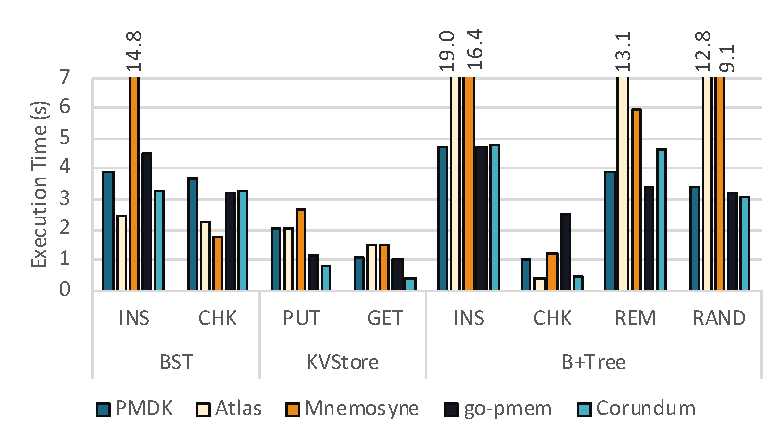
\includegraphics[width=3.3in]{Graphs/perf.pdf}
    \end{center}
    \caption{\label{fig:perf} Performance comparison between \this{}, PMDK, Atlas, Mnemosyne, and go-pmem}
\end{figure}

Wordcount measures scalability.  \This{} provides
a separate allocator and journal object for every thread to allow concurrency. %concurrent allocation.
\reffig{fig:scal} confirms that the performance scales with thread count.
When the allocator cannot find a free block in its free lists, it deliberates the task to another allocator which is protected by a lock.

\begin{figure}
    \begin{center}
    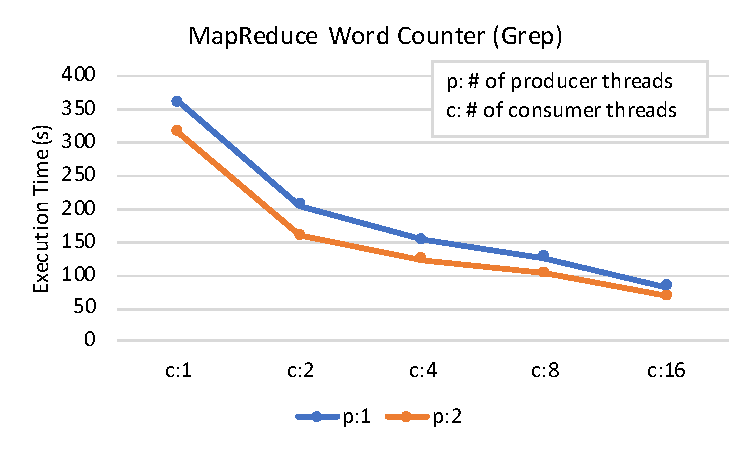
\includegraphics[width=3.3in]{Graphs/scal.pdf}
    \end{center}
    \caption{\label{fig:scal} \this{}'s scalable performance with regard to the number of threads. The baseline is running one producer and one consumer object sequentially (seq).}
\end{figure}
%auto-ignore
\section{Related Work}
\label{sec:related}


\ignore{This section needs quite a bit of work. You need to think through what the key claims are for \this{}'s novelty and then layout how we differ from other systems.

  Novelty:

  1.  static checks for almost all PM safety properties.  Dynamic for the rest.  Some libraries provide some of this.

  2.  PL and compiler support.  What other compiler-based PM tools are there?  what does the compiler do?  Note that we dont really have PM compiler support.  We just have a language that has lots of useful tool.  I think most of the compiler support is about inserting logging calls at the right place.  Interestingly, doing so in Rust would be non-idiomatic.   What about at the language level (I think its just NVM direct)?  How are we different better than them?

  3. I'm not sure what pronto and pangolin have to do with this \this{}.  We dont address the challenges that pangolin fixes.   Pronto is a pm library, but that's where the relevence ends.
  
}

Many projects have addressed the challenges of PM programming with
software~\cite{pmdk,pronto,mnemosyne,nvheaps,atlas,oracle-nvm-direct,ido,usnap,cohen2018object,
  autopersist,janus,libpm,lazypersist,pisces} and/or
hardware~\cite{ogleari2018steal,Kiln,jeong2018efficient,xu2020hardware}.
\reftab{tab:libs} highlights the checks some of these systems provide.  The systems not listed in table
provide fewer checks (in some cases this is by design).

In response, several projects provide
testing~\cite{pmtest,oukid2016testing,xfdetector} and debugging
tools~\cite{intel-pmemcheck,intel-inspector,lantz2014yat} targeting PM systems.
While useful, these tools cannot provide safety guarantees and they rely on the
programmer using them reliably and providing tests with good coverage.

\subsection{PM Programing Libraries}

Among PM libraries, PMDK~\cite{pmdk} is the mostly widely used.  It provide dynamic checks to prevent inter-pool pointers in C and the C++ version provides static enforcement for atomicity, but otherwise the programmer is responsible for enforcing safety.

NV-Heaps~\cite{nvheaps} and Mnemosyne~\cite{mnemosyne} rely on the C++ type system and a custom compiler, respectively, to statically avoid data races, atomicity violations, and pointers from PM into volatile memory.  Both systems go to some pains help avoid bugs, but the weakness of the C/C++ type systems make the guarantees they provide easy to circumvent.  NV-heaps addresses the problem of closed pools -- by not allowing pools to close.

NVM Direct~\cite{oracle-nvm-direct} adds extensions to C/C++ via a custom compiler that gives the programmer detailed control over logging.  It is, by design, ``dangerously flexible - just like C''~\cite{personalbillbridge} to enable as many manual optimizations as possible, so it relies heavily on the programmer to enforce safety properties.  \This{} opts for safety over flexibility and does not require specific compiler support.

\subsection{Orthogonal Persistence}

Orthogonal persistence is a principle for programmability enhancement historically developed for databases which may yield an imperfect implementation of persistent data in terms of performance in persistent programming. To follow orthogonal persistence, the persistence abstraction should allow the creation and manipulation of data in an identical manner, regardless of its lifetime Thereby the persistent view of information is integrated with the programming language view~\cite{atkinson1995orthogonally}. 
None of the mentioned libraries in this paper provides orthogonal persistence.

Following orthogonal persistence principle, Atlas~\cite{atlas} integrates failure-atomicity with thread-safety, and provides an identical view for manipulating both volatile and persistent data using locks. However, the creation of persistent data is different from volatile data.

Similarly, go-pmem~\cite{gopmem} uses native pointers to provide persistent programming in Go~\cite{golang}. Although it uses native pointers, it requires the programmer to use transactions in order to enhance the performance.

\This{} targets safety with minimal performance overhead, so it may slightly sacrifice programmability in some senses. To make data type orthogonal to persistence, we need compiler-level passes to add dynamic checks such as persistence identification, many of which, such as network sockets and thread handles, are inherently transient. Rather than this, we allow only \csym{PSafe} types to reside in PMEM, and enforce a transactional interface for data manipulation.


%are two of the first PM libraries that offer a safe programming environment by enforcing some invariants statically. NV-Heaps also uses reference counting for garbage collection while it should be done manually in Mnemosyne. Although many of the invariants hold statically, checking that data is PM safe is a loophole in both of them. Also, the pool isolation check happens in the runtime, and the safety of V-to-NV pointers is not fully guaranteed.

%Atlas~\cite{atlas} introduces failure-atomic sections (FASE) in which data consistency is guaranteed if the user correctly integrate it. Atlas uses a combination of compiler (static) and runtime (dynamic) support to ensure the recoverability of data within a FASE. Atlas provides means to implement a safe PM program, but does not enforce PM safety.


% PMDK~\cite{pmdk}, NV-Heaps~\cite{nvheaps}, Mnemosyne~\cite{mnemosyne}, and
% NVM-Direct~\cite{oracle-nvm-direct} provide libraries for using PM by
% leveraging failure-atomic transactional memory techniques.  Unlike \this{},
% these systems require the programmer to carefully include the provided APIs to
% accurately access the PM. On the contrary, \this{} hides the PM programming
% requirements underneath standard programming with smart pointers.

% Atlas~\cite{atlas} and NVthreads~\cite{nvthreads} guarantee failure-atomicity
% in multi-thread PM programming by using locks on persistent objects and memory
% pages, respectively. Similarly, \this{} provides transaction wide \csym{Mutex}
% to allow concurrent access to the shared persistent data.

% Pronto~\cite{pronto} uses Asynchronous Semantic Logging to add
% failure-atomicity to the volatile data structures with regards to PM
% programming. Using Pronto, the user develops the data structure to records the
% operation semantics in PM and replays it when a crash happens to reconstruct
% the data structure back to the latest snapshot. Similar to other libraries,
% failure to using it correctly and thoroughly may result in untraceable bugs.

% Log-Structured NVMM~\cite{log-nvmm} suggests swapping the log and data to
% reduce the write traffic and the number of barriers. \This{} also uses this
% technique to save one of the two required flushing operation for updating a
% persistent object.

%auto-ignore
\section{Conclusion}
\label{sec:conclude}

\This{} enforces PM safety invariants mostly using static checks.  It,
therefore, eliminates memory management, pointers safety, and logging bugs and
avoids the attendant costs of testing, debugging, fixing, and recovering from
them.  It accomplishes this using Rust's type system to carefully control when
the program can modify persistent and volatile state and when and where mutable
references to persistent state can exist.  Our experience shows that \this{} is
relatively easy to use and our measurements show that \this{}'s performance is
comparable with (or better than) existing PM libraries.

\section*{Acknowledgement}

This work was supported in part by Semiconductor Research Corporation (SRC)
and by NFS award 1629395.
%auto-ignore
%\newpage
\bibliographystyle{ACM-Reference-Format}
\bibliography{libpaper/common,paper}


%%%%%%%%%%%%%%%%%%%%%%%%%%%%%%%%%%%%%%%%%%%%%%%%%%%%
% When adding this appendix to your paper, 
% please remove above part
%%%%%%%%%%%%%%%%%%%%%%%%%%%%%%%%%%%%%%%%%%%%%%%%%%%%
% \clearpage 
\appendix
\section{Artifact Appendix}

%%%%%%%%%%%%%%%%%%%%%%%%%%%%%%%%%%%%%%%%%%%%%%%%%%%%%%%%%%%%%%%%%%%%%
\subsection{Abstract}

This appendix provides the necessary information for obtaining the source code,
building, and running performance and functionality tests of Corundum. 
We describe the hardware and software requirements to run the
experiments and reproduce the results as they appear in \refsec{sec:results}.

\subsection{Artifact check-list (meta-information)}

{\small
\begin{itemize}
  \item {\bf Program: } Corundum library and its unit tests, Rust, Cargo, PMDK v1.8, Atlas, Mnemosyne, and go-mem. Input files for the experiments are included (74~MB).
  \item {\bf Compilation: } \This{}: Rust 1.52.0-nightly (publicly available); PMDK, Atlas, Mnemosyne: GNU C++11, CMake $>=$ 3.3; go-pmem: Go lang.
  \item {\bf Data set: } Data set is included (Will be downloaded automatically)
  \item {\bf Run-time environment: } Linux (tested in Ubuntu 20.04, Fedora 27, and NixOS). The NVMM should be mounted in \verb+/mnt/pmem0+ using a DAX-enabled file system (e.g. EXT4-DAX). We also provide a docker image containing Ubuntu 20.04 LTE with pre-installed dependencies.
  \item {\bf Hardware: } A machine with a 16-core Intel processor with 32 GB or larger NVMM (e.g. Optane DC). The docker does not require NVMM and uses DRAM to emulate NVMM. The ISA should provide \verb+CL_FLUSHOPT+ since we customized Atlas to use it instead of \verb+CL_FLUSH+. Other libraries are adaptable to the system configuration.
  \item {\bf Metrics: } Execution time
  \item {\bf Output: } Numerical results stored in \verb+perf.csv+, \verb+scale.csv+, and \verb+micro.csv+ for performance, scalability, and micro-benchmarks, respectively. Expected results are also included in the text.
  \item {\bf Experiments: } A script is provided to run the experiments and generate results. Although the results may vary depending on the build and the environment, there should not be a big difference.
  \item {\bf How much disk space required (approximately)?: } 32~GB
  \item {\bf How much time is needed to prepare workflow\linebreak(approximately)?: } 30 minutes.
  \item {\bf How much time is needed to complete experiments (approximately)?: } $\leq$ 1 hour.
  \item {\bf Publicly available?: } Code, unit-tests, documentation, examples, and evaluation scripts are publicly available.
  \item {\bf Code licenses (if publicly available)?: } Apache v2.0
  \item {\bf Archived (provide DOI)?: } \href{https://zenodo.org/record/4539743}{DOI: 10.5281/zenodo.4539743}
\end{itemize}

%%%%%%%%%%%%%%%%%%%%%%%%%%%%%%%%%%%%%%%%%%%%%%%%%%%%%%%%%%%%%%%%%%%%%
\subsection{Description}

\subsubsection{How to access}

The artifacts are publicly available
through Zenodo archival repository and GitHub. You can access the code by using its \href{https://zenodo.org/record/4321062}{DOI} or cloning the GitHub repository at \href{https://github.com/NVSL/Corundum/}{https://github.com/NVSL/Corundum/}.
We also prepared a Docker image available at DockerHub (\href{https://hub.docker.com/r/mhz88/corundum}{mhz88/corundum:latest}).

\subsubsection{Hardware dependencies}

We recommend running the experiments on a machine with a physical persistent memory such as Intel Optane DC with at least 32~GB available space.

Also, the scalability test requires a 16-core processor to measure the execution time while running threads in parallel.

\subsubsection{Software dependencies}

\begin{itemize}
  \item To install \This{} without running the evaluations, installing Rust compiler with Cargo tool (1.52.0-nightly) would suffice.
  \item To measure performance, we use \verb+perf+ (>=4.9.215), a linux (kernel>=3.10.0) builtin monitoring tool for analyzing programs (automated installation is included in `\verb+eval/ubuntu-deps.sh+').
  \item If you wish to use Docker, please install Docker and use the prepared docker image with pre-installed dependencies. Otherwise, please run os specific setup scripts (e.g `\verb+eval/ubuntu-deps.sh+' on Ubuntu latest version).
  \item `\verb+eval/build.sh+' compiles and installs other libraries and workloads for comparison. It internally calls `\verb+build.sh+' scripts for each individual library (can be found in `\verb+eval/pmdk+', `\verb+eval/atlas+',\linebreak`\verb+eval/mnemosyne+', and `\verb+eval/go+').
\end{itemize}

\subsection{Installation}

The docker image already has the dependencies pre-installed. If you wish to run it on a real system, please follow the steps in the rest of this section.

\subsubsection{Installing Rust}

If you prefer installing Rust manually rather than running `\verb+ubuntu-deps.sh+', please follow through these steps.
On a Unix-like OS machine, the following commands
install Rust compiler, Cargo, and \verb+rustup+. 

\begin{verbatim}
$ curl --proto '=https' --tlsv1.2 \
     -sSf https://sh.rustup.rs | sh
$ source $HOME/.cargo/env
$ rustup default nightly
\end{verbatim}

% If tou are using
% another OS, please refer to Rust's official website
% for the instructions at
% \begin{center}
%   \href{https://www.rust-lang.org/tools/install}{https://www.rust-lang.org/tools/install}
% \end{center}

\subsubsection{Building Corundum}

Corundum is publicly available in GitHub. Please use
the following commands to clone and compile it.

\begin{verbatim}
$ git clone https://github.com/NVSL/Corundum.git
$ cd Corundum
$ cargo build --release --examples
\end{verbatim}

\subsubsection{Verifying the compilation}

Optionally you can run the tests to verify it.
Since tests may share pool files, we run them sequentially.

\begin{verbatim}
$ cargo test --tests -- --test-threads=1 
\end{verbatim}

%%%%%%%%%%%%%%%%%%%%%%%%%%%%%%%%%%%%%%%%%%%%%%%%%%%%%%%%%%%%%%%%%%%%%
\subsection{Experiment workflow}

Running the experiments is automated though the following set of commands:

\begin{verbatim}
$ sudo sysctl -w kernel.perf_event_paranoid=-1
$ git clone https://github.com/NVSL/Corundum.git
$ cd Corundum/eval
$ ./ubuntu-deps.sh  # Install dependencies
$ ./build.sh        # Build the libraries and workloads
$ ./run.sh -o       # Run the tests with CLFLUSHOPT
$ ./results.sh      # Display the results
\end{verbatim}

The \verb+eval/ubuntu-deps.sh+ downloads necessary dependencies, and \verb+eval/build.sh+ compiles the benchmark applications.
\verb+eval/run.sh+ executes benchmarks and collects the results, and generates three files:

\begin{itemize}
  \item \verb+perf.csv+: Compares Corundum with other libraries (\reffig{fig:perf})
  \item \verb+scale.csv+: Evaluates multi-threading scalability (\reffig{fig:scal})
  \item \verb+micro.csv+: Lists average latency for basic operations (\reftab{tab:microbench})
\end{itemize}

\noindent Finally, \verb+eval/results.sh+ displays the results on screen.


\subsection{Evaluation on Docker}

We also prepared a docker image with pre-installed dependencies, PMDK (libpmemobj and libpmemobj-cpp), Atlas, Mnemosyne, go-pmem, Corundum, and the input datasets. To emulate PM using DRAM, we bind \verb+/dev/shm+ to a directory inside the docker (i.e. `\verb+-v /dev/shm:/mnt/pmem0+'). To use real PM, you may mount it to a folder as explained in \refsec{sec:custom}, and then replace \verb+/dev/shm+ in the command line arguments with the mount point directory (e.g. \verb+-v /mnt/pmem0:/mnt/pmem0+). We also need to enable \verb+perf_event_open+ system calls. Please run the following commands on the host machine to give permission to, download, and run the docker image.


\begin{verbatim}
$ sudo sysctl -w kernel.perf_event_paranoid=-1
$ wget https://raw.githubusercontent.com/NVSL/
Corundum/main/eval/docker-default.json
$ docker run --security-opt \
    seccomp=./docker-default.json \
    -v /dev/shm:/mnt/pmem0 \
    -it mhz88/corundum:latest bin/bash
\end{verbatim}
% docker run --security-opt \
%     seccomp=./docker-default.json \
%     --mount type=tmpfs,destination=/mnt/pmem0 \
%     -it mhz88/corundum:latest bin/bash

\noindent
Inside the docker, use the following commands to run the experiments:

\begin{verbatim}
$ cd ~/Corundum/eval
$ ./run.sh && ./results.sh
\end{verbatim}

%%%%%%%%%%%%%%%%%%%%%%%%%%%%%%%%%%%%%%%%%%%%%%%%%%%%%%%%%%%%%%%%%%%%%
\subsection{Evaluation and expected results}

We discuss performance evaluation in terms of execution time compared with equivalent implementations in PMDK, Atlas, Mnemosyne, go-pmem, and execution time using multiple threads to show its scalability. 

\subsubsection{Performance}

To compare Corundum's performance with other libraries, we use three applications: BST, VKStore, and B+Tree. The provided script runs these applications automatically with random inputs. The results are stored in \verb+perf.csv+ and should look like \reftab{tbl:perf}. Please modify other library installations as needed since we do not guarantee them.

\begin{table}
  \center
  \small
  \setlength\tabcolsep{1.5pt}
  \caption{Expected output for performance comparison between Corundum and a selection of other libraries (\csym{perf.csv}). \reffig{fig:perf} graphically represetns this data.}
  \label{tbl:perf}
  \begin{tabular}{|r|c|c|c|c|c|c|c|c|} \hline
    \multicolumn{9}{|c|}{Execution Time (s)}	\\ \hline						
    & \multicolumn{2}{|c|}{BST}	& \multicolumn{2}{|c|}{KVStore}&\multicolumn{4}{|c|}{B+Tree}	     \\\hline	
    & INS&CHK&PUT&GET&INS&CHK&REM&RAND           \\\hline
    PMDK     &3.9&5.3&2.1&1.1&4.7&1.0&3.9&3.4    \\\hline
    Atlas    &2.5&2.3&2.0&1.5&20.6&0.4&13.0&11.9 \\\hline
    Mnemosyne&14.0&1.8&2.5&1.5&14.9&1.2&6.0&8.5  \\\hline
    go-pmem  &4.6&3.2&1.1&1.0&4.6&2.5&3.4&3.2    \\\hline
    Corundum &3.3&3.1&0.8&0.4&4.8&0.5&4.6&3.1    \\\hline
  \end{tabular}
\end{table}


\subsubsection{Scalability}
To verify that Corundum provides scalability with respect to the number of threads, we implemented a MapReduce application called \verb+grep+ (referred as \verb+wordcount+ in the text) which counts the frequency of every word in a list of text documents. The producer threads fill up a shared stack, and the consumer threads pop a segment from the stack and count the number of appearance of every words in the segment locally. We do not collect the local records because it adds a fixed amount of execution time to sequentially fetch data from threads. This is to better evaluate the scalability of the library. \reftab{tbl:scale} (\reffig{fig:scal}) shows the expected speedup in execution time for various number of producer (p) and consumer (c) threads. We use Large Canterbury Corpus (http://www.data-compression.info/Corpora/CanterburyCorpus/) dataset as the input files (included in the archive).

\begin{table}[!ht]
  \caption{Expected output for Scalability (scale.csv) using emulated PM. \reffig{fig:scal} graphically represents this data.}
  \label{tbl:scale}
  \begin{tabular}{|c|c|c|c|c|c|c|c|} \hline
    seq&1:1&1:2&1:3&1:4&1:5&1:6&1:7\\\hline
    1.0&1.4&2.9&4.1&5.2&6.2&7.4&8.7\\\hline\hline
    1:8&1:9&1:10&1:11&1:12&1:13&1:14&1:15\\\hline
    9.5&11.1&12.3&13.2&14.2&15.0&15.7&15.9\\\hline
  \end{tabular}
\end{table}


\subsubsection{Microbenchmarks}
The run script also reproduces \reftab{tab:microbench}. To measure the latency of each individual operation, we use a Rust provided measurement tool called \csym{Instant} and \csym{Duration}. On Linux, it internally uses \cfunc{clock\_gettime} system call. Since this tool is not zero cost, for operations with low latency such as \csym{Deref}, we measure running a batch of 50k of them and then calculate the average number. For these operations, we cannot report standard deviation.

%%%%%%%%%%%%%%%%%%%%%%%%%%%%%%%%%%%%%%%%%%%%%%%%%%%%%%%%%%%%%%%%%%%%%
\subsection{Experiment customization}
\label{sec:custom}

Corundum requires a DAX-enabled file system. We recommend EXT4-DAX. If you run the experiments on a real machine, use the following commands to format and mount the drive (assuming the device name is \verb+/dev/pmem0+):

\begin{verbatim}
$ sudo mkdir /mnt/pmem0
$ sudo mkfs.ext4 /dev/pmem0
$ sudo mount -t ext4 -o dax /dev/pmem0 /mnt/pmem0
$ sudo chmod -R 777 /mnt/pmem0
\end{verbatim}

If there is no pmem device available, you may emulate it using DRAM though the following instructions:

\begin{verbatim}
$ sudo mkdir /mnt/pmem0
$ sudo mount -t tmpfs /dev/pmem0 /mnt/pmem0
\end{verbatim}

Many of the latency components are originated in Hardware, such as using \verb+CL_FLUSHOPT+ instead of \verb+CL_FLUSH+ when available. Corundum does not automatically detect these capabilities. However, it comes with some builtin features. In `\verb+Cargo.toml+', under the `features' section, update \verb+default=[]+ or use `\verb+--features="..."+' argument as required. For example, if the system supports \verb+CLWB+ instructions, you may force Corundum to use that by changing the default features to this:

\begin{center}
  \verb+default = ["use_clwb"]+
\end{center}

%%%%%%%%%%%%%%%%%%%%%%%%%%%%%%%%%%%%%%%%%%%%%%%%%%%%%%%%%%%%%%%%%%%%%
\subsection{Methodology}

Submission, reviewing and badging methodology:

\begin{itemize}
  \item \url{https://www.acm.org/publications/policies/artifact-review-badging}
  \item \url{http://cTuning.org/ae/submission-20201122.html}
  \item \url{http://cTuning.org/ae/reviewing-20201122.html}
\end{itemize}

%%%%%%%%%%%%%%%%%%%%%%%%%%%%%%%%%%%%%%%%%%%%%%%%%%%%
% When adding this appendix to your paper, 
% please remove below part
%%%%%%%%%%%%%%%%%%%%%%%%%%%%%%%%%%%%%%%%%%%%%%%%%%%%



\end{document}
